\pdfminorversion=7
\documentclass[11pt]{article}
\PassOptionsToPackage{round,authoryear,longnamesfirst,sort}{natbib}
\usepackage[natbibapa]{apacite}
\usepackage[T1]{fontenc}
\usepackage[utf8]{inputenc}
\usepackage{lmodern}
\usepackage{amsmath,amssymb,bm}
\usepackage{siunitx}
\sisetup{per-mode=symbol,range-phrase=--,range-units=single}
\DeclareSIUnit\ppm{ppm}
\DeclareSIUnit\rpm{r/min}
\DeclareSIUnit\bar{bar}
\DeclareSIUnit\year{yr}
\usepackage[margin=2.5cm]{geometry}
\usepackage{graphicx}
\usepackage{booktabs}
\usepackage{array}
\usepackage{multirow}
\usepackage{longtable}
\usepackage{caption}
\usepackage{enumitem}
\usepackage{xcolor}
\usepackage[round,authoryear]{natbib}
\usepackage[hidelinks]{hyperref}
\usepackage{microtype}

\newcommand{\RESULTTODO}[1]{\textbf{[RESULT TO BE ADDED: #1]}}
\newcommand{\CITETODO}[1]{\textbf{[CITATION TO BE RESOLVED: #1]}}
\newcommand{\TODO}[1]{\textbf{[TODO: #1]}}
\newcommand{\COMPANION}[1]{\emph{(companion manuscript, submitted separately: #1)}}

\newcommand{\Xh}{X_{\mathrm{h}}}            % total n-hexane loading
\newcommand{\Xw}{X_{\mathrm{w}}}            % total water loading
\newcommand{\Xc}{X_{\mathrm{c}}}            % critical (constant-/falling-rate) loading
\newcommand{\Xe}{X_{\mathrm{e}}}            % equilibrium loading
\newcommand{\Xf}{X_{\mathrm{f}}}            % attached/interparticle solvent holdup
\newcommand{\Wret}{W}                       % retained (sorbed) loading
\newcommand{\Wcap}{W_{\mathrm{cap}}}        % retained-water evidence capacity
\newcommand{\ah}{a_{\mathrm{h}}}
\newcommand{\aw}{a_{\mathrm{w}}}
\newcommand{\yh}{y_{\mathrm{h}}}
\newcommand{\yw}{y_{\mathrm{w}}}
\newcommand{\Nt}{N_{\mathrm{t}}}            % total (Stefan) molar flux
\newcommand{\JE}{J_{E}}                     % total interfacial energy flux
\newcommand{\front}{s}                      % front radius
\newcommand{\frontz}{z}                     % front coordinate z=(s/R)^3
\newcommand{\Rp}{R_{\mathrm{p}}}            % particle radius
\newcommand{\Deff}{D_{\mathrm{eff}}}
\newcommand{\rhodm}{\rho_{\mathrm{dm}}}     % dry composite meal density in particle
\newcommand{\epsp}{\varepsilon_{\mathrm{p}}}% particle porosity
\newcommand{\epsb}{\varepsilon_{\mathrm{b}}}% bed porosity
\newcommand{\Tint}{T_{\Gamma}}              % interface temperature
\newcommand{\jump}[1]{\left[\!\left[ #1 \right]\!\right]}
\newcommand{\Rey}{\mathrm{Re}}
\newcommand{\Pra}{\mathrm{Pr}}
\newcommand{\Sci}{\mathrm{Sc}}
\newcommand{\Nu}{\mathrm{Nu}}
\newcommand{\Le}{\mathrm{Le}}
\newcommand{\Bi}{\mathrm{Bi}}
\newcommand{\Pe}{\mathrm{Pe}}
\newcommand{\DT}{DT}                        % desolventizer--toaster
\newcommand{\DC}{DC}                        % dryer--cooler

\newcommand{\FanerDryTime}{88.1}
\newcommand{\FanerCrossTwenty}{46.6}
\newcommand{\FanerFallingInterval}{17.7}
\newcommand{\FanerExitHexane}{0.00161}
\newcommand{\FanerExitWater}{0.0144}
\newcommand{\FanerExitTemperature}{114.4}
\newcommand{\FanerFreeEnd}{46.8}
\newcommand{\FanerFallingShortfall}{30}
\newcommand{\FanerMaxBeta}{0.639}
\newcommand{\FanerLastHolderClockTemperature}{114.0}
\newcommand{\DTFiniteHexaneDry}{135}
\newcommand{\DTFiniteHexaneWet}{111}
\newcommand{\DTFiniteMoisture}{18.2}
\newcommand{\DTFiniteTemperature}{105.0}

\usepackage{xr}
\externaldocument[S-]{supplementary_submission}
\usepackage{multicol}
\usepackage{float}

\newcommand{\Xhwa}{X_{\mathrm{h,w}}^{a}}         % historical wet-core hexane label
\newcommand{\Lwh}{L_{\mathrm{wh}}^{\mathrm{eff}}}% binary pore mobility
\newcommand{\Lwr}{L_{\mathrm{w,ret}}^{\mathrm{eff}}}% retained-matrix mobility
\newcommand{\Kws}{K_{\mathrm{w,s}}}              % retained-water surface coefficient
\newcommand{\Cdm}{\rho_{\mathrm{dm,p}}}          % dry composite meal density in the particle
\newcommand{\wo}{w_{\mathrm{o}}}                 % residual-oil mass fraction of dry meal
\newcommand{\woref}{w_{\mathrm{o,ref}}}
\newcommand{\Bh}{B_{\mathrm{h}}}                 % hexane binding potential
\newcommand{\qnet}{q_{\mathrm{net}}}
\newcommand{\Tg}{T_{\mathrm{g}}}
\newcommand{\Tb}{T_{\mathrm{b}}}
\newcommand{\dd}{\mathrm{d}}

\renewcommand{\topfraction}{0.90}
\renewcommand{\bottomfraction}{0.80}
\renewcommand{\textfraction}{0.07}
\renewcommand{\floatpagefraction}{0.80}
\setcounter{topnumber}{3}
\setcounter{bottomnumber}{2}
\setcounter{totalnumber}{4}
\setlength{\textfloatsep}{10pt plus 2pt minus 2pt}
\setlength{\intextsep}{10pt plus 2pt minus 2pt}
\setlength{\floatsep}{8pt plus 2pt minus 2pt}
\setlength{\abovecaptionskip}{4pt}
\captionsetup{font=small}

\begin{document}

\title{A particle model of hexane removal and water uptake in soybean meal
desolventizing}

\author{Tom\'a\v{s} Svoboda$^{1,3,*}$, Marcela Slukov\'a$^{1}$, Svatopluk Henke$^{1}$, Tom\'a\v{s} Moucha$^{2}$\\[6pt]
\parbox{0.88\textwidth}{\raggedright\normalsize
$^{1}$University of Chemistry and Technology Prague, Department of Carbohydrates and Cereals, Technick\'a 5, 166~28 Prague 6, Czech Republic\\[2pt]
$^{2}$University of Chemistry and Technology Prague, Department of Chemical Engineering, Technick\'a 5, 166~28 Prague 6, Czech Republic\\[2pt]
$^{3}$Siemens, s.r.o., Digital Industries, Siemensova 1, 155~00 Prague, Czech Republic\\[2pt]
$^{*}$Corresponding author: \texttt{tomas3.svoboda@vscht.cz}}}

\date{}

\maketitle

\noindent\textbf{Running title:} Hexane desolventization of meal

\begin{abstract}
In a desolventizer-toaster (DT), steam desolventization of oilseed meal
couples hexane removal, water uptake and heat transfer. We formulate a
conservative particle model containing free liquid hexane, binary pore
gas, retained water and hexane, and a separate external water film.
Component and energy jump conditions determine how the liquid-hexane
interface recedes; after the core disappears, the same inventories
continue to evolve in a stationary radial particle. Published
thermodynamic and retention properties, together with declared transport
coefficients, parameterize the model. Converged discrete calculations
conserve water, hexane and energy through all three regimes. The
formulation is exercised in two prescribed baths, in which the
surrounding gas history is specified rather than solved. In the first, a
water-bearing soybean particle in Faner's pure-hexane vapour at
\SI{120}{\celsius} falls from 0.20 to 0.10 kg hexane/kg dry meal in
\SI{\FanerFallingInterval}{\second}, compared with 25.4 s measured. The
source reports preheating, but not the exact initial temperature,
moisture or mass-weighted particle sizes. In the second, a particle
followed through a 1766.5-s prescribed DT history leaves with 18.2\%
wet-basis moisture, 111 ppm wet-basis hexane and a mean temperature of
\SI{105.0}{\celsius}. The particle response is benchmarked against available literature
experiments and published industrial outlet ranges, without fitting the
falling-rate trajectories or DT outlet values. This common formulation
provides the particle-level basis for a DT digital twin that can shorten
process design and support model-based control.
\end{abstract}

\noindent\textbf{Keywords:} desolventization; soybean meal; n-hexane;
moving-front model; sorption; food process modeling

\paragraph*{Practical Applications.}
A prescribed-bath experiment lets a process engineer examine solvent
loss, moisture uptake and temperature without first solving a complete
desolventizer-toaster (DT). The same particle equations describe a
pure-hexane drying experiment and a steam-rich DT scenario. In the
pure-hexane case, the calculated particle dries faster than the measured
charge; better size, exposure and temperature information is needed to
explain the difference. In the DT case, the particle reaches 18.2\%
wet-basis moisture with liquid-water imbibition included; the uptake rate
rests on one same-material measurement. The model returns signed water,
hexane and energy fluxes that can later be coupled to conservative tray
balances.

\section{Introduction}\label{sec:intro}
Solvent extraction leaves oilseed meal wet with hexane. In a
desolventizer-toaster (DT), live steam strips the solvent while heated trays
supply additional energy \citep{sipos1961dt,witte_nd_soybeanmeal,karnofsky1985recovering}.
Residual solvent matters for safety and emissions; condensed water must
later be removed, and the meal's thermal history affects protein
quality \citep{epa1995ap42,kemper2013solvent,mustakas1981critical}.
The engineering question is how to supply enough heat and residence time
for solvent removal and toasting without excessive steam use, later
drying duty or damage to meal quality \citep{kemper2013solvent,witte_nd_soybeanmeal}.
A particle model must therefore connect solvent removal, moisture uptake
and heat transfer throughout the transition from externally wetted meal
to a particle containing only retained material and pore gas.

These processes are coupled. Evaporation consumes energy at the particle
surface or an internal liquid boundary. Incoming steam can condense, and
both retained water and residual hexane contribute to storage and transport.
Liquid-water imbibition also differs from vapour sorption. Experiments on soy
protein isolates show that imbibition combines sorption, capillarity and
interstitial retention, whereas vapour sorption describes a different
hydration experiment \citep{jovanovich2003wateruptake}.
Those measurements motivate treating liquid contact separately from vapour
exposure; their capacities and rates cannot be transferred directly
to hot, hexane-bearing extracted meal.

Published desolventization models emphasize different parts of this
sequence. The superheated-hexane experiments and receding-front model of
\citet{faner2019kinetics} describe a heat-fed liquid-hexane core. The transport
account of \citet{cardarelli2002modeling} resolves a diffusion-controlled
drying tail. \citet{coletto2022modeling} couples a transient radial particle
to a steady axial bed in the diffusion-controlled zone, treating the
preceding flashing zone separately. Here we combine component and energy
conservation at a receding liquid-hexane interface with binary pore gas,
matrix retention and a separately conserved external water film.
After the core disappears, the same stored components and energy continue
to evolve in a stationary radial particle.

In the first of two prescribed baths, a water-bearing particle in pure
superheated hexane is compared with the soybean experiment of
\citet{faner2019kinetics}; pure supplied vapour does not imply a
water-free meal. In the second, a particle is followed from feed
through a prescribed steam-rich DT history. Prescribing the bath isolates
the particle response, so the surrounding vapour composition and
temperature need not be predicted. In a future coupled tray calculation,
the signed water, hexane and energy fluxes would enter the gas and tray
balances, which would determine the next local bath state.

The two comparisons rest on different kinds of evidence. In the Faner
experiment, the measured constant-rate duty informs external heat
supply; later loading and temperature readings provide the comparisons.
Faner reports preheating in the apparatus and particle-size summaries, but
not the exact initial temperature, initial meal moisture or a mass-weighted
size histogram. The DT history is an engineering scenario; published outlet
ranges provide process context rather than measurements of the same
particle and operating point. Liquid-water imbibition is part of the particle
formulation, and its transport coefficients are declared rather than
measured. Numerical verification and complete time integration make
these assumptions inspectable; independent measurements are needed to
establish their predictive accuracy.

The paper has two goals: to state one conservative particle formulation
and to exercise it in both baths.
Section~\ref{sec:model} defines the particle equations and phase regimes,
and Section~\ref{sec:numerics} their numerical integration, admissibility
checks and verification. Section~\ref{sec:validation} presents the two
experiments, Section~\ref{sec:discussion}
discusses their meaning for DT practice and the measurements needed next,
and Section~\ref{sec:conclusions} concludes. The
Supplementary Material contains detailed source readings, parameters,
numerical evidence and the separate scalar Fickian comparison with the
earlier Faner measurements.

\section{Particle model}
\label{sec:physical}
\label{sec:model}
\label{sec:thermo}

This section states the particle model that the rest of the paper
exercises: the phase regimes of one particle, the balances in each region,
the conditions that close the moving front and the properties that enter
them. Readers mainly interested in the process results can read
Section~\ref{sec:physical:regimes} and then continue with
Section~\ref{sec:validation}.

\subsection{Particle geometry, inventories and phase regimes}
\label{sec:physical:regimes}
\label{sec:physical:threshold}
\label{sec:physical:inversion}
\label{sec:physical:lewis}

The model follows one particle through three regimes, defined by where
liquid hexane remains. Hexane is stored as external free hexane, hexane in a
liquid-hexane core, retained hexane and pore gas.
External free hexane wets the surface in regime A. Its depletion allows the
liquid-hexane core to recede in regime B, leaving a dry shell. Throughout
this paper, \emph{dry shell} means depleted of free liquid hexane, not free
of water or retained hexane. Regime C begins when the liquid-hexane core
disappears. Steam can form an external water film, from which
\emph{liquid-water imbibition} transfers water into the particle's retained-water
inventory. Retained water includes effective matrix and interstitial
retention; it does not imply that all water is molecularly bound.

We approximate the particle by a porous sphere of fixed radius $\Rp$.
This geometry resolves radial heat and mass transport with one length
scale, as in the particle descriptions of \citet{faner2019kinetics} and
\citet{cardarelli2002modeling}. Actual meal particles are irregular;
the radius selected for each experiment is therefore stated with its
source and interpretation. Fixed radius and porosity separate transport
from swelling and shrinkage, for which no constitutive laws are supplied here.
The particle's total n-hexane loading $\Xh$ (every loading here in
\si{\kilogram} per \si{\kilogram} of dry, water- and solvent-free meal)
is compared with two thermodynamic reference loadings at the particle's
temperature. The first is the critical loading $\Xc(T)$, at which mobile
liquid stops reaching the outer surface; it is set on the transition loading
\citet{faner2019kinetics} measured (Table~\ref{tab:parameters}). The second is the equilibrium loading
$\Xe^{*}(T,P)$, at which no condensed hexane remains. The star denotes
evaluation at the pressure-feasible saturated activity $a^{*}$ of
Eq.~\eqref{eq:aceiling}. In regime~A, while external free hexane remains,
bulk liquid wets the outer surface at unit hexane activity and the resistance
is external. In regime~B ($0<\front<\Rp$), liquid is present only behind a
receding interface, and removal is limited by the heat reaching that interface
through a growing dry shell. In
regime~C, no liquid-hexane core remains: $\front=0$. Retained material and
pore gas continue to obey the same local component and energy balances.
Core extinction is a geometric conservation event; a particle-mean loading
is not used to prescribe it. The saturated equilibrium loading is a
thermodynamic reference rather than a uniform-particle transition rule
(Figure~\ref{fig:schematic}).

\begin{figure}[htbp]
\centering
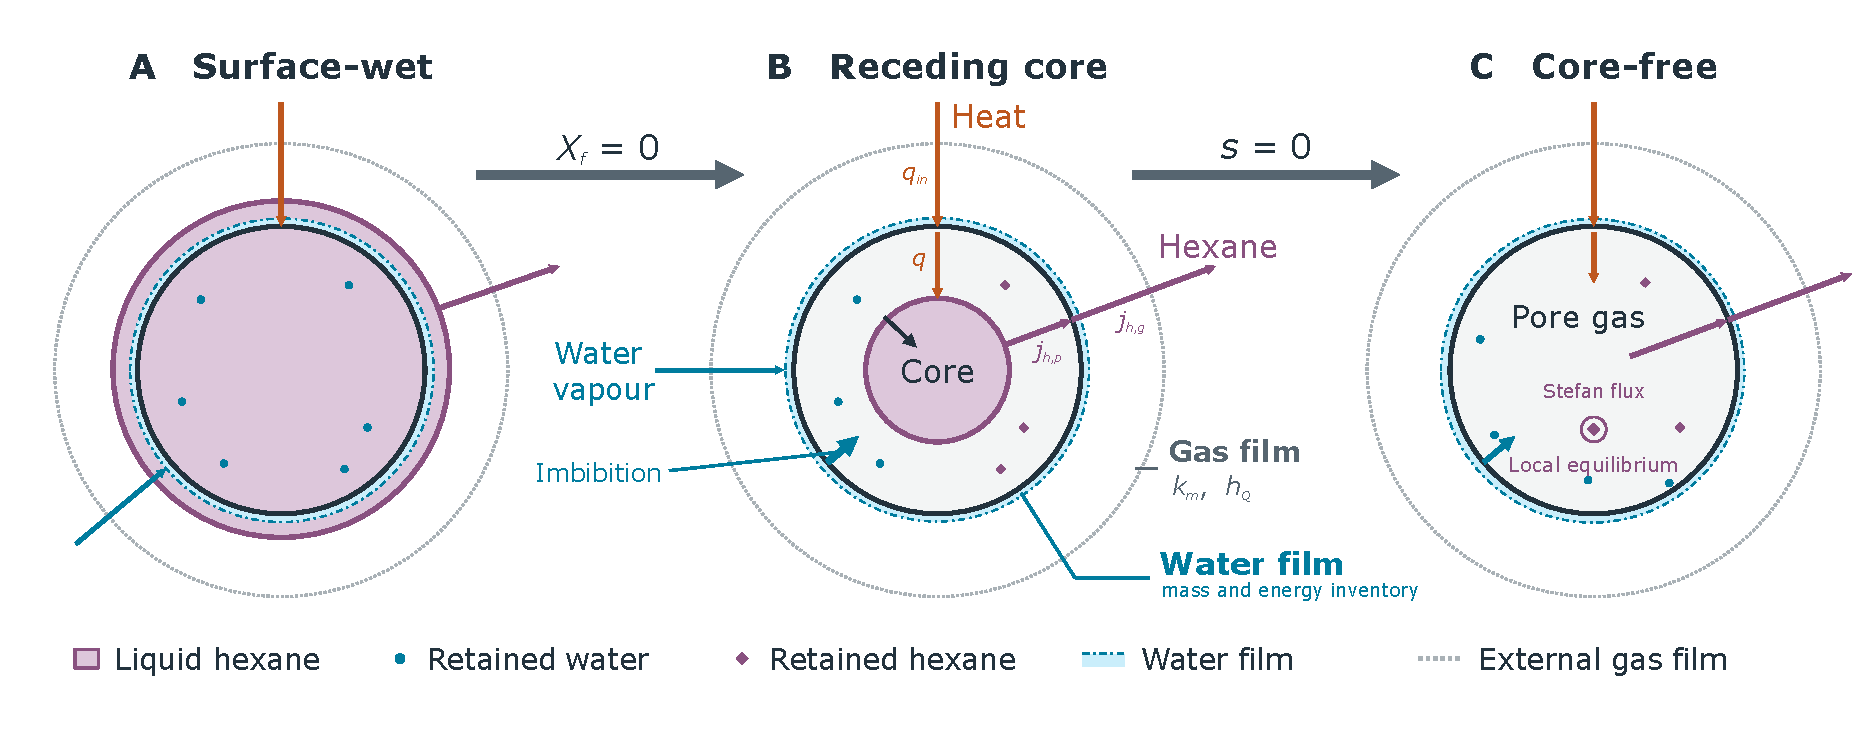
\includegraphics[width=\textwidth]{figures/fig_particle_model.pdf}
\caption{Particle regimes and transport pathways.}
\label{fig:schematic}
\end{figure}

Figure~\ref{fig:schematic} follows external free-hexane depletion
($\Xf=0$) and subsequent core disappearance ($\front=0$).
Purple represents hexane and blue represents water; orange arrows show
incoming heat. The dashed blue band is the optional external water film,
through which hexane can escape in the proposed closure. Liquid-water
imbibition operates in the dry shell connected to that film, with no
additional liquid-water flux into the liquid-hexane core. Dots and diamonds
represent retained water and retained hexane, respectively. Geometry and
film thickness are schematic. Fluxes are outward-positive: $j$ is
mass-based and $N$ molar, with $h_k^{\mathrm{mass}}=\bar h_k/M_k$;
subscripts p and g identify the particle and gas sides of the surface.

The particle model is written so that it can later be coupled to a tray
model. For prescribed gas and heat-transfer conditions, the particle balances return
outward-positive surface fluxes $j_{\mathrm{w}}(\Rp)$,
$j_{\mathrm{h}}(\Rp)$ and $\JE(\Rp)$ on one caloric datum. These are
responses to the evolving interior, rather than imposed drying rates. For
particle classes $c$ with total exposed areas $A_{\mathrm{ex},c}$, the rates
delivered to a future tray gas balance would be
$\sum_c A_{\mathrm{ex},c}j_{k,c}(R_{p,c})$ for component $k$ and
$\sum_c A_{\mathrm{ex},c}J_{E,c}(R_{p,c})$ for total energy. Condensation has a
negative water rate; each gas source has an equal and opposite entry in
the particle balance. The tray would return its updated gas state to the particles.
In this paper, the gas and bed conditions along the equipment trays are
prescribed instead. This separates the particle response from countercurrent
gas mixing and tray residence, which is useful for testing the particle equations before
coupling them to DT design calculations; steam consumption itself requires
those equipment balances \citep{kemper2013solvent}.

The equilibrium boundary is evaluated at the \emph{pressure-feasible} hexane
activity
\begin{equation}
a^{*}(T,P) \;=\; \min\!\left(1,\;P/P_{\mathrm{sat}}^{\mathrm{h}}(T)\right),
\label{eq:aceiling}
\end{equation}
with $P$ the total pressure and $P_{\mathrm{sat}}^{\mathrm{h}}$ the n-hexane
vapour pressure, both in pascals. Equation~\eqref{eq:aceiling} is an
ideal-mixture diagnostic. The pore and interface equilibrium used in the
calculations uses binary-virial gas fugacities and the pure-liquid equation-of-state
fugacities on the same pressure and caloric datum. It does not omit those
corrections when locating phase boundaries. Above the solvent's
boiling point at the bed pressure, an equilibrium loading taken at unit
activity is overstated. Evaluated with
\eqref{eq:aceiling}, the two boundaries stay one to two orders of magnitude
apart and separate further as the temperature rises; the paper uses only that
\emph{ordering} (Sec.~\ref*{S-sup:regime}).

The A--B transition occurs when the external free-hexane inventory
$\Xf$ is exhausted. While $\Xf>0$, liquid wets the surface and the front stays at
$\front=\Rp$; once $\Xf=0$, it may recede and leave a dry shell. This
sequential-drainage condition is stated in Eq.~\eqref{eq:complementarity}.
The reference critical loading of
\SI{0.20}{\kilogram\per\kilogram} measured by
\citet{faner2019kinetics} sets the effective critical-volume capacity
at the reference liquid density, 615 kg/m$^3$. At the particle's actual
temperature, $\Xc(T)=\kappa_v\varepsilon_{\mathrm g}
\rho_{\mathrm{h,l}}(T,P)/\Cdm$, with $\kappa_v=2.675$ fixed by that
reference capacity. The liquid density comes from the same equation of
state used in the component and energy balances. The depletion loading
therefore has a prescribed temperature dependence, while the time at which
it is reached follows from the regime-A inventory balance under the
prescribed gas and heat history. The component and energy jumps then determine the recession speed
and the dry-side hexane flux at the front. The shell balances and surface
conditions determine the corresponding particle-surface exchanges. In the
discrete model the front first departs over
an accepted time step, giving a finite shell thickness without assigning the
shell the width of one radial cell (Sec.~\ref*{S-sup:item27}). The A--B
boundary is thus a surface-state constraint, with no fitted time or drying-rate
selector. The stationary binary regime-C closure starts after the liquid-hexane core
has vanished. In a calculation, the crossing \emph{loading} therefore
reproduces a supplied value; the crossing \emph{time} is the tested
prediction, conditional on the external history
(Section~\ref{sec:validation:faner}).

Heat must first cross the gas-side resistance and then the dry shell to
reach the receding front. In the reported scale comparison, the external
thermal resistance dominates until the core radius falls to about
$0.28\Rp$; the dry-shell resistance dominates later
(Sec.~\ref*{S-sup:closures}). The present total-vapour closure adds no
pressure-driven transport resistance, so front recession is heat-limited.
This distinction matters when interpreting falling-rate data: the 2019
Faner records support a heat-limited description, whereas the older
Faner records and the mechanism of \citet{cardarelli2002modeling} support
a diffusion-limited description. The separate scalar Fickian comparison
in Eq.~(\ref*{S-eq:ficklimit}) represents the latter; it does not replace
the shared particle law in either experiment
(Sec.~\ref*{S-sup:tworegimes}).

Temperature and composition also vary over different radial scales. The
dry-shell Lewis number of $223.25$ requires their profiles to be
reconstructed separately near the moving front
\citep{crank1956diffusion,perre2023stateoftheart}.

\subsection{Local balances and region closures}
\label{sec:model:geometry}
\label{sec:model:local}
\label{sec:model:wet}
\label{sec:model:dry}

Inside each region the model is a set of conservation laws with no source
terms, closed differently in the liquid-hexane core and in the dry shell. The sphere
holds two conserved mobile components, water and n-hexane, and an immobile
composite dry meal of local density $\Cdm$ with a residual-oil mass
fraction $\wo$. A sharp interface at radius $r=\front(t)$, with $t$ the time,
separates a liquid-hexane core ($\mathrm{w}$) from a dry shell ($\mathrm{d}$); the
region label $\alpha$ takes either value. Radial fluxes are positive
outward, and recession means $\dot{\front} < 0$. The total radial energy flux is
defined once, on both sides, as
$\JE^{\alpha} = q^{\alpha} + \sum_{k} \bar{h}_{k}^{\alpha} j_{k}^{\alpha}$,
with $q$ the conductive heat flux, $j_{k}$ the radial flux of component $k$
and $\bar{h}_{k}$ the partial molar enthalpy on the common datum of
Section~\ref{sec:thermo:datum}. In each smooth region
\begin{align}
\frac{\partial C_{k}^{\alpha}}{\partial t}
 + \frac{1}{r^{2}}\frac{\partial}{\partial r}\!\left(r^{2} j_{k}^{\alpha}\right)
 &= 0, \qquad k \in \{\mathrm{w},\mathrm{h}\},
\label{eq:localcomp}\\[2pt]
\frac{\partial u^{\alpha}}{\partial t}
 + \frac{1}{r^{2}}\frac{\partial}{\partial r}\!\left(r^{2} \JE^{\alpha}\right)
 &= 0,
\qquad j_{\mathrm{dm}} = 0, \qquad j_{L_{\mathrm{o}}} = 0 ,
\label{eq:localenergy}
\end{align}
with $C_{k}$ the total local concentration of component $k$ over all of its
phases, $u$ the total local internal energy density, and $j_{\mathrm{dm}}$
and $j_{L_{\mathrm{o}}}$ the fluxes of the immobile dry meal and residual oil.
Retention,
evaporation and condensation redistribute a component between local phases and
are therefore \emph{not} sources in \eqref{eq:localcomp}: no phase-change term
appears in the smooth-region equations (Sec.~\ref*{S-sup:ale}).

Two statements close the liquid-hexane core. First, no relative n-hexane flux is carried inside
the mobile-liquid region: at activation, every material shell stores the
historical label $\Xhwa = \Xc(\theta_{a})$, the critical loading at its
temperature at activation $\theta_{a}$, and thereafter
\begin{equation}
\frac{\mathrm{D}_{s}}{\mathrm{D}t}\!\left(\Cdm\,\Xhwa\right) = 0
\label{eq:shellconserved}
\end{equation}
following the solid. Thus $\Xhwa$ is the apparent mobile-liquid hexane
loading of the liquid-hexane core, stored at activation and distinct both from the
particle's total loading $\Xh$ and from the retained hexane of the dry
shell. The core is liquid-filled, the hexane activity is unity,
and the non-negativity of the mobile liquid is an admissibility condition, not
a clipped quantity. Second, the core is resolved, not lumped, with specific energy
per kilogram of dry meal
\begin{equation}
e_{\mathrm{w}} \;=\; h_{\mathrm{dm}}(T,\wo)
 \;+\; \Xw\, h_{\mathrm{w,l}}(T,P)
 \;+\; \Xhwa\, u_{\mathrm{h,l}}(T,P)
 \;-\; \Bh(\ah{=}1,T,\wo),
\label{eq:wetenergy}
\end{equation}
with $h_{\mathrm{dm}}$ the specific enthalpy of the dry meal, $\Xw$ the total
water loading, and $h_{\mathrm{w,l}}$ and $u_{\mathrm{h,l}}$ the specific
enthalpy of liquid water and the specific internal energy of liquid n-hexane,
both in \si{\joule\per\kilogram}. Retained and mobile hexane are not
carried separately in this energy, so the binding
potential $\Bh$ is counted once and the repartition between them is source-free.

The dry shell stores each component in two forms, pore gas and a retained
contribution, with distinct storage terms and distinct thermodynamics; no
retained-only symbol includes pore gas. Transport
consists of one thermodynamic-force pore flux, one retained-matrix water flux and one
algebraic total flux,
\begin{align}
J_{\mathrm{w}} \;=\; -J_{\mathrm{h}}
 &\;=\; -\Lwh\,\nabla_{\mathrm{comp}}\!\left[\frac{\mu_{\mathrm{w}}-\mu_{\mathrm{h}}}{RT}\right],
\label{eq:binaryflux}\\[2pt]
N_{\mathrm{w,ret}}
 &\;=\; -\Lwr\,\nabla_{\mathrm{comp}}\!\left[\frac{\mu_{\mathrm{w,ret}}}{RT}\right],
\qquad
N_{i}^{\mathrm{g}} = y_{i}\Nt + J_{i} ,
\label{eq:retflux}
\end{align}
with $\mu_{\mathrm{w}}$ and $\mu_{\mathrm{h}}$ the pore-gas chemical potentials
of water and n-hexane and $\mu_{\mathrm{w,ret}}$ that of retained water
(\si{\joule\per\mole}), $R$ the gas constant, $\Lwh$ and $\Lwr$ the pore and
retained-matrix mobilities (\si{\mole\per\meter\per\second}), $y_{i}$ the
pore-gas mole fraction of component $i$, and the fluxes $J_{i}$,
$N_{\mathrm{w,ret}}$, $N_{i}^{\mathrm{g}}$ and $\Nt$ molar
(\si{\mole\per\meter\squared\per\second}). The total (Stefan) flux $\Nt$ is recovered algebraically from the summed
continuity equations rather than fitted. It rests on an Onsager mobility whose
degeneracy vanishes exactly at either purity and needs no composition floor
\citep{krishna1997maxwell}. The shell energy flux carries each stream exactly
once, with no latent, binding, pressure-volume or Stefan-energy correction on
top (Sec.~\ref*{S-sup:stefanrecovery}). We retain composition-driven mass transport and conductive heat transport,
and neglect independent Soret terms because no thermal-diffusion
coefficients for this meal are supplied. This is a constitutive approximation;
it does not show that thermal diffusion is negligible. Here $\nabla_{\mathrm{comp}}$ denotes the composition part of the
fixed-$(T,P)$ chemical force, not the full gradient of a temperature-dependent
standard chemical potential. At ordinary faces, the isothermal
composition secant is evaluated at a common face temperature. The moving-interface
reconstruction integrates that composition derivative along the actual
linear temperature/composition path,
\begin{equation}
G_{\mathrm{comp}}(\Xi)=\frac{1}{d}\int_0^1
\left.\frac{\partial\Xi}{\partial y_{\mathrm h}}\right|_{T(\lambda),P}
\frac{\dd y_{\mathrm h}}{\dd\lambda}\,\dd\lambda,
\qquad \Xi=\ln(f_{\mathrm w}/f_{\mathrm h})
\ \hbox{or}\ \ln(f_{\mathrm w}/f_{\mathrm{ref}}).
\end{equation}
Here $d$ is the face separation and $f_i$ is the equation-of-state fugacity.
Energy transport remains non-isothermal and includes component enthalpies.
This is the declared nominal transport approximation in both prescribed-bath experiments.
The pressure variation omitted by
taking $\Nt$ from continuity is estimated from Darcy's law across the dry
shell,
\begin{equation}
\Delta P \;\approx\; \frac{\Nt\, R T}{P}\,\frac{\mu_{g}}{B}\,(\Rp-\front),
\label{eq:darcy}
\end{equation}
with $\mu_{g}$ the pore-gas viscosity and $B$ the Darcy permeability.
For an illustrative vapour-flux bound, take
$|\Nt|=\SI{0.5}{\mole\per\square\metre\per\second}$; this is a supplied
sensitivity scale, not the measured or calculated mean flux of the new DT
history. With this flux bound,
$\mu_{g}=10^{-5}\,\si{\pascal\second}$, $T$ at the heteroazeotrope and a
shell \SI{1}{\milli\metre} thick, the estimate gives $\Delta P$ of about
\SI{0.15}{\kilo\pascal}, \SI{1.5}{\kilo\pascal} and \SI{15}{\kilo\pascal}
at $B=10^{-12}$, $10^{-13}$ and $10^{-14}\,\si{\square\metre}$. A capillary
bundle $B=\varepsilon_{g} r_{\mathrm{pore}}^{2}/(8\tau)$ at the particle
porosity $0.14$ and a tortuosity of three is about
$10^{-13}\,\si{\square\metre}$ for a \SI{5}{\micro\metre} pore
($\Delta P$ about \SI{1}{\kilo\pascal} on the same bound) and about
$6\times 10^{-15}\,\si{\square\metre}$ for a \SI{1}{\micro\metre} pore
($\Delta P$ about \SI{25}{\kilo\pascal}). Below about
$10^{-15}\,\si{\square\metre}$ the estimate exceeds the bed pressure.
The isobaric closure therefore assumes that the vapour crosses a
connected pore space of several micrometers. It does not apply to a path
confined to sub-micrometer pores, and no measured permeability
of this meal is supplied here.
These fluxes do not reduce to a scalar Fick law for n-hexane.
Summing \eqref{eq:retflux} over the two components gives
$N_{\mathrm{w}}^{\mathrm{g}} + N_{\mathrm{h}}^{\mathrm{g}} = \Nt$, fixed by
continuity and not by a gradient. With the mobility
$\Lwh = c\,\yw\yh D_{b}$, where $c$ is the molar density of the pore gas and $D_{b}$
the binary pore coefficient, \eqref{eq:binaryflux} becomes a binary Fick law
with coefficient $D_{b}$ only at zero total flux and constant total
concentration. In a pure n-hexane pore gas the binary flux vanishes, and the n-hexane
flux is $\Nt$ itself (Secs.~\ref*{S-sup:stefanrecovery} and~\ref*{S-sup:singlecomponent}).
The scalar Fick description used for the older drying records is a
separate comparison with an effective transport coefficient, given in
Eq.~(\ref*{S-eq:ficklimit}). In both prescribed baths, regime~C instead
integrates the stationary radial binary component and total-energy balances.
Its initial inventories and temperatures come from the conservative
core-extinction projection. The same particle equations therefore carry
solvent removal through core disappearance and the remaining drying tail.

The value of the coupled formulation lies in its accounting; it does not
claim that one coefficient represents every possible falling-rate
mechanism. Water and n-hexane share the pore-gas and energy balances, while
water in the retained matrix has its own transport path and retained hexane
contributes to both storage and binding energy. A change in the rate of
evaporating hexane therefore also changes the heat carried out, the
temperature and the conditions under which water can condense or desorb;
none can be added as an independent source after solving a hexane-only
particle. The immobile wet-core liquid and the sorbate in the dry shell are
distinct inventories. While the front is still moving, recession is limited
by heat. After the front vanishes, regime~C carries the remaining hexane
in the same stationary binary radial model. Equation~(\ref*{S-eq:ficklimit}) is the radial
problem used for the comparison with the slower literature curves. The comparison does
not establish that the heat-limited front and the diffusion-limited tail
are asymptotic branches of one fully identified rate law.

\begin{samepage}
\subsection{Front conditions}
\label{sec:model:front}

The front conditions fix the front velocity from the heat that reaches the
front. For a spherical control volume with moving inner and outer radii
$r_1(t)$ and $r_2(t)$, conservation of either component and of total energy
requires
\begin{align}
\frac{\dd}{\dd t}\left(4\pi\int_{r_1}^{r_2} C_k r^2\,\dd r\right)
 &=-4\pi r_2^2(j_k-\dot r_2 C_k)_{r_2}
   +4\pi r_1^2(j_k-\dot r_1 C_k)_{r_1},
 \qquad k\in\{\mathrm{w},\mathrm{h}\},
\label{eq:movingcomp}\\[2pt]
\frac{\dd}{\dd t}\left(4\pi\int_{r_1}^{r_2} u r^2\,\dd r\right)
 &=-4\pi r_2^2(\JE-\dot r_2 u)_{r_2}
   +4\pi r_1^2(\JE-\dot r_1 u)_{r_1}.
\label{eq:movingenergy}
\end{align}
The terms proportional to $\dot r_1$ and $\dot r_2$ account for material
swept through the moving boundaries. Shrinking this volume onto
$r=\front(t)$ gives the Rankine--Hugoniot conditions for both components
and total energy \citep{crank1984free},
\begin{align}
\jump{\,j_{k} - \dot{\front}\,C_{k}\,}_{\mathrm{w}}^{\mathrm{d}} &= 0,
\qquad k \in \{\mathrm{w},\mathrm{h}\},
\label{eq:rhcomp}\\[2pt]
\jump{\,q + \textstyle\sum_{k} \bar{h}_{k} j_{k} - \dot{\front}\,u\,}_{\mathrm{w}}^{\mathrm{d}} &= 0 ,
\label{eq:rhenergy}
\end{align}
\end{samepage}
with $\jump{\cdot}_{\mathrm{w}}^{\mathrm{d}}$ the dry-side value minus the
wet-side value. Two different wet-side states occur in
these conditions and must be kept apart. The first is the equilibrium
interface trace, which the interface conditions solve for. The second is the
\emph{donor} state, the one-sided limit of the wet-core fields themselves.
Every term multiplying $\dot{\front}$ is a stored state, swept at the state
of its own side. With the zero
wet-side relative hexane flux of \eqref{eq:shellconserved}, the hexane jump
fixes the dry-side flux that the moving front produces,
\(j_{\mathrm{h,d}}=\dot{\front}\bigl(C_{\mathrm{h,d}}^{\Gamma}-C_{\mathrm{h,w}}^{\mathrm{b}}\bigr)\).
The wet-side donor value, the historical label stored at activation rather
than a re-solved critical loading, must exceed the dry-side trace.
Substituting this flux into \eqref{eq:rhenergy} moves the term
\(\bar{h}_{\mathrm{h,d}} j_{\mathrm{h,d}}\), which is proportional to
\(\dot{\front}\), into the denominator. The front velocity is then
\begin{equation}
\dot{\front} \;=\;
 -\,\frac{
   \jump{q}_{\mathrm{w}}^{\mathrm{d}}
   + \bar{h}_{\mathrm{w,d}}\, j_{\mathrm{w,d}}
   - \bar{h}_{\mathrm{w,w}}\, j_{\mathrm{w,w}}
 }{
   \bar{h}_{\mathrm{h,d}}\bigl(C_{\mathrm{h,d}}^{\Gamma}
    - C_{\mathrm{h,w}}^{\mathrm{b}}\bigr)
   - \bigl(u_{\mathrm{d}}^{\Gamma} - u_{\mathrm{w}}^{\mathrm{b}}\bigr)
 } ,
\label{eq:frontvelocity}
\end{equation}
a heat-supply to stored-state-jump quotient in its donor-restricted form.
The numerator is the conduction jump, dry side minus wet side, plus the
enthalpy carried by the water flux. That water flux is evaluated from the
water jump and the shell. The denominator is the energy required to sweep a
volume of liquid-hexane core into the dry-side state. On the common datum of
Section~\ref{sec:thermo:datum} it contains the latent heat of the hexane
removed, a smaller ideal-gas correction and the binding energy already stored
in \(u\) (Sec.~\ref*{S-sup:ale}). The superscript \(\Gamma\) marks the
equilibrium interface trace, \(\mathrm{b}\) the donor state, and
\(\bar{h}_{\mathrm{h,d}}\) the partial enthalpy of n-hexane on the dry side. This
is where a heat limit and a transport limit could meet in one expression. In
this formulation they do not. The dry-side flux is not throttled by
\eqref{eq:binaryflux}, which carries only the separation of the two vapours,
and the total flux is algebraic. The numerator, the heat reaching the
front through the film and the dry shell in series, therefore sets the front
velocity wherever the vapour is swept outward faster than the two vapours
separate. In a march inside the band, the shell P\'eclet numbers are of order
$10^{3}$ (Sec.~\ref*{S-sup:regimegrid}). A transport-controlled recession
needs a finite resistance on the total flux. Equation~(\ref*{S-eq:ficklimit})
would supply one, but this formulation does not apply it at the moving front:
the front velocity contains no Darcy or Knudsen term. Regime~C begins only
after that front has vanished and retains the binary radial closure.
The model contains no rate selector, no
minimum of a diffusion rate and a heat rate, and no empirical evaporation-rate
law.

\subsection{Admissible states and the removal of swept material}
\label{sec:model:interface}
\label{sec:model:regimeA}
\label{sec:model:donor}

The front conditions hold in the discrete model only if states outside the
admissible set are rejected and swept material is removed at one consistent
state. The interface is closed by continuity of temperature, local phase
equilibrium at unit hexane activity on the wet side, and equal liquid and gas
pressure; the last condition means that macroscopic capillarity is omitted. Admissibility is a complementarity
system rather than a clipping rule,
\begin{equation}
\Xf \ge 0, \qquad \Rp - \front \ge 0, \qquad \Xf\,(\Rp-\front) = 0,
\qquad \dot{\front} \le 0 ,
\label{eq:complementarity}
\end{equation}
whose first three conditions express strict sequential drainage (the
external free-hexane loading $\Xf$ must be exhausted before the front may
leave the outer surface) and whose fourth restricts the formulation to
primary drainage. A trajectory that violates any of them, inverts the
interfacial concentration jump or loses interior mobile liquid is rejected
at that step. The violated bound is reported and the last accepted state
is left unchanged: no second interface is created and no state is repaired
to keep the integration running.

One consistency requirement needs a separate statement, because a
discretization can violate it silently. When the interface sweeps material,
the concentration and the energy density used to debit the swept volume must
be read from the same material state. Using the equilibrium trace for one and
the consumed material's bulk state for the other would imply a pre-drainage
that the intraparticle P\'eclet number of this system excludes. Both are
therefore taken at the bulk, old-time state of the consumed piece. In that
state the retained water is \emph{continuous} across the front, because hexane
drains and water does not (Sec.~\ref*{S-sup:donor}). The formal statement is a gauge covariance: shifting the
arbitrary caloric zero of water by a constant $c_{\mathrm{w}}$ must move the
discrete energy residual of the interface rows by exactly $c_{\mathrm{w}}$
times their discrete water residual,
\begin{equation}
\frac{\partial R_{E}}{\partial c_{\mathrm{w}}} \;=\; R_{\mathrm{w}} ,
\label{eq:gauge}
\end{equation}
identically in the discrete state. Section~\ref{sec:verification} uses
this identity as the acceptance test for the interface treatment. The same
test is available to any moving-boundary phase-change discretization: if
the energy residual does not move exactly with the component residual when
that component's caloric zero is shifted, latent or binding heat is being
counted twice, or the swept material is being debited from the wrong state.

\subsection{The conserved external water film}
\label{sec:model:waterfilm}

When the bath supplies condensing water, the model stores it in an
external water film, an inventory separate from retained water. Steam condensation supplies heat
for desolventization while increasing the water that may require removal
in the downstream dryer \citep{kemper2013solvent,witte_nd_soybeanmeal}.
Keeping the film separate lets the balances determine how much water enters
the particle and how much evaporates back to the bath. We use one film
temperature and inventory at the surface, rather than resolving its liquid
flow or spatial thickness. Let $L_{\mathrm w}$ be its mass per
unit particle area, $j_{k,\mathrm p}$ the outward pore-side component flux,
and $j_{k,\mathrm g}$ the outward gas-film flux. To isolate the effect of
water uptake, the external water film is assumed to add no resistance to
hexane escape. This limiting case is not a measured water-film permeability;
a blocking effect would require an additional constitutive law.
The surface balances are
\begin{align}
\frac{\dd L_{\mathrm w}}{\dd t}
 &=j_{\mathrm w,\mathrm p}-j_{\mathrm w,\mathrm g},\\
0&=j_{\mathrm h,\mathrm p}-j_{\mathrm h,\mathrm g},\\
\frac{\dd[L_{\mathrm w}u_{\mathrm w,l}(T_{\mathrm s})]}{\dd t}
 &=J_{E,\mathrm p}-J_{E,\mathrm g}.
\label{eq:externalwaternode}
\end{align}
The gas-film closure uses an ideal binary mass-coordinate partition,
with equation-of-state phase traces and partial enthalpies. For total outward
mass flux $j_t$, conductance $K_f=\rho_f k_m$, and hexane mass fractions
$Y_{\mathrm h,s}$ and $Y_{\mathrm h,b}$,
\begin{align}
j_{\mathrm h,g}&=Y_{\mathrm h,s}j_t+
 K_f(Y_{\mathrm h,s}-Y_{\mathrm h,b})\Phi(j_t/K_f),\qquad
j_{\mathrm w,g}=j_t-j_{\mathrm h,g},\\
\Phi(x)&=\frac{x}{e^x-1},\quad \Phi(0)=1,\qquad
\beta=\frac{j_{\mathrm w,g}c_{p,\mathrm w}^{f}+
 j_{\mathrm h,g}c_{p,\mathrm h}^{f}}{h_Q},\\
q_{\mathrm{in}}&=h_Q\Phi(\beta)(T_{\mathrm b}-T_{\mathrm s}),\qquad
J_{E,\mathrm g}=-q_{\mathrm{in}}+
 \sum_k\frac{j_{k,\mathrm g}}{M_k}\bar h_k(T_{\mathrm s}).
\end{align}
The component heat capacities are component partial-enthalpy secants between
surface and bulk temperatures. Both component capacity fluxes enter
$\beta$, including counter-diffusion. The same analytic Ackermann
expression is used within a declared band $|\beta|\le3$. Its largest
accepted value in the recorded calculations is 1.2063, above the previously
assessed film band $|\beta|\le1$. This wider band is a declared assumption
about the film law, separate from the numerical root tolerances; it has not
been demonstrated for this gas film.
All advected partial enthalpies enter the two total-energy fluxes once.
Positive external liquid selects unit surface water activity; with zero
liquid, gas-side composition is solved from the same three balances and
may remain undersaturated. Appearance and depletion are conservative
events, not resets of the film mass or temperature. The interior retention
capacity is a separate active set. The numerical unit-activity trace of the
hexane-transparent film and its sensitivity are stated with the experiments.
For the regime-A surface in the pure-hexane bath, the hexane-only surface
active set sets the outward water flux to zero while external free hexane
remains. The water in the particle stays stored and becomes exposed through
the binary pore gas once the external free hexane is depleted.


\subsection{Liquid-water imbibition from the external water film}
\label{sec:model:liquidcontact}
Liquid-water imbibition is assumed to occur when the external water film
contacts the dry shell. Steam condenses on the particle faster than the
water can move inward, so a liquid film accumulates on the surface and is
drawn into the pore structure afterwards, where the matrix and the
interstitial space retain it \citep{karnofsky1985recovering}. Liquid
contact also admits water that vapour sorption does not: the imbibition
capacity of soy protein isolates exceeds their vapour-sorption capacity
several-fold \citep{jovanovich2003wateruptake}. We represent this path
as an effective finite-conductance pathway into the existing
capacity-bounded retained-water inventory. The closure does not identify
every absorbed molecule as strongly bound and adds no independently
resolved pore-liquid domain. Vapour transport and retention remain active
through the original component equations.

Let $\psi=\ln a_{\mathrm{w,ret}}$ be the activity potential evaluated from
the actual retained-water state. For the additional liquid-water mobility
$\mathcal L_\ell>0$, liquid contact conductance $K_\ell>0$ and distance $d>0$
between the outer cell and surface trace, the external contribution is
\begin{equation}
G_\ell=\left(\frac{d}{\mathcal L_\ell}+\frac{1}{K_\ell}\right)^{-1},
\qquad N_\ell=-G_\ell(\psi_{\mathrm s}-\psi_{\mathrm p}).
\label{eq:finitecontact}
\end{equation}
$N_\ell$ is outward-positive in mol/(m$^2$ s). Thus
$0<G_\ell\le K_\ell$ and $G_\ell\to K_\ell$ as $d\to0$:
when the dry shell first forms, the surface conductance stays finite.
Interior faces in the dry shell use $G_\ell=\mathcal L_\ell/d$.
This added path is absent at the remaining wet-core interface and when
external liquid is absent. Surface and cell activities follow their
capacity-bounded retained states; the added force is not obtained by
substituting unit pure-liquid activity for the retained surface trace.

For available film stock $L_{\mathrm w,old}$, inward addition is limited by
\begin{equation}
j_{\ell,\mathrm{in}}\le
\max\!\left(0,\frac{L_{\mathrm w,old}}{\Delta t}
+j_{\mathrm w,\mathrm p}^{\mathrm{base}}-j_{\mathrm w,\mathrm g}\right).
\label{eq:liquidstocksupply}
\end{equation}
The final flux enters $j_{\mathrm w,\mathrm p}$ in
Eq.~\eqref{eq:externalwaternode} and the particle balance with opposite
signs. Its donor retained-water partial enthalpy enters the energy flux
once. Under the negligible-Soret approximation for this additional path,
its composition-force dissipation is proportional to
$R G_\ell(\psi_{\mathrm s}-\psi_{\mathrm p})^2\ge0$.
Liquid-water imbibition is an effective transport hypothesis, not a
resolved capillary-pressure, hydraulic saturation or swelling model.
Water displacement of pore hexane is neglected, and the film adds no
resistance to hexane escape (Section~\ref{sec:model:waterfilm}).

Two coefficients set the rate: the liquid contact conductance $K_\ell$ at
the wetted surface and the liquid-water mobility $\mathcal L_\ell$ inside
the shell. They act in series, so an uptake measurement on one particle
size fixes only their combination. We therefore set the mobility first
and derive the conductance from the one same-material measurement that
exists. The mobility is 1000 times the reference retained-water mobility
$\Lwr$. In porous hygroscopic solids the liquid transport coefficient
rises by about three orders of magnitude between the dry state and
water-filled pores \citep{kunzel1995simultaneous}; we apply the
water-filled end of that range because the path is active only while a
liquid film wets the shell. Above a factor of about 300 the calculation
no longer depends on this choice, because the surface then controls the
uptake. A tenfold increase from 1000 to 10\,000 moves the DT outlet
moisture by 0.07 percentage points; a tenfold decrease moves it by 0.58
(Sec.~\ref*{S-sup:contactscale}). The conductance is then set from
the only kinetic measurement of solvent-extracted soybean meal in liquid
water: 1.4-mm particles at \SI{80}{\celsius} are saturated within the
first 90-s sample \citep{hemmingsen2008water}. Reproducing that time
with Eq.~\eqref{eq:finitecontact} and the retention law of
Eq.~\eqref{eq:luikov}, and scaling to \SI{100}{\celsius} by the viscosity
of water, gives $K_\ell=0.32$ mol/(m$^2$ s) (construction in
Sec.~\ref*{S-sup:contactscale}). With the adopted mobility, the
resistance length $\mathcal L_\ell/K_\ell$ is 2.6 mm, 1.8 times the DT
particle radius. Surface entry therefore carries about two thirds of the series
resistance at that radius, and a contact-only sphere at the DT radius
fills from the feed loading to within 0.01 kg/kg of capacity in about
150 s. The value rests on declared transfer assumptions (a sphere of the
sieve size, interior saturation at the first sample, viscosity scaling)
and is not a measurement on DT meal. Neither coefficient was adjusted to
the DT outlet, which is governed by the condensate supply and the
retention capacity (Sec.~\ref*{S-sup:contactsensitivity}).

\subsection{One caloric datum per component}
\label{sec:thermo:datum}

One numerical zero per component makes every latent and binding heat appear
once and gives the energy balance an acceptance test. Every state function of
a component is evaluated on \emph{one} numerical zero shared by all of its
phases: mobile core liquid, external free hexane, the retained phase, pore
gas and bulk vapour alike. Two consequences follow. First, latent and binding
effects occur exactly once, through differences of stored state plus the
component enthalpy fluxes the energy flux already carries. A separate
vaporization-enthalpy source, a fitted sorption-heat source or a power-law
excess sorption enthalpy is therefore excluded, not merely unnecessary,
because it would count the same energy twice. Second, because the zero is
arbitrary, it must cancel: shifting it may change no temperature, flux,
reported quantity or external energy residual. This property becomes the
acceptance test of Section~\ref{sec:verification}. For hexane, the caloric consequences of retention follow
from its temperature-dependent isotherm: the integrated sorption potential, the net heat of sorption and the
binding potential $\Bh$ of \eqref{eq:wetenergy} form a Gibbs--Helmholtz pair
whose two routes must agree (Sec.~\ref*{S-sup:binding}).
The nominal retained-water energy uses liquid-water enthalpy on the same
datum. Its temperature-independent Luikov activity law contributes no
separate excess water-binding heat. Condensation and evaporation energy
are already present through phase-state differences and component fluxes.

\subsection{Sorption isotherms, property equations and parameters}
\label{sec:thermo:properties}
\label{sec:thermo:gab}
\label{sec:thermo:binding}

The sorption isotherms and property equations close the model, and the
ranges over which they were measured set where its results can be trusted.
Retained n-hexane on reference soybean meal follows the
Guggenheim--Anderson--de Boer isotherm fitted by \citet{cardarelli1996hexane},
\begin{equation}
W_{\mathrm{native}}(\ah,T) = \frac{X_{m}\,C\,x}{(1-x)\,(1-x+C\,x)},
\qquad x = K(T)\,\ah,
\label{eq:gab}
\end{equation}
with $X_{m}$ the monolayer loading and $C$ and $K$ the dimensionless GAB
constants. Both $C$ and $K$ have an Arrhenius temperature dependence, and
no activity clamp is applied. The
sorbing sample carried reference oil, so \eqref{eq:gab} is a \emph{total-meal}
isotherm, with no duplicate oil inventory at the reference oil fraction
$w_{\mathrm{o,ref}}=0.0195$. For an off-anchor oil fraction the existing
reference-anchored composite closure is
\begin{equation}
W_{\mathrm{h}}=\alpha_o W_{\mathrm{h,native}}+\beta_o q_o(a_{\mathrm h}),
\quad \alpha_o=\frac{1-w_o}{1-w_{\mathrm{o,ref}}},\quad
\beta_o=\frac{w_o-w_{\mathrm{o,ref}}}{1-w_{\mathrm{o,ref}}},\quad
q_o=0.9635a_{\mathrm h}^{2.7036}.
\end{equation}
The same weights give dry-composite heat capacity
$\alpha_o c_{p,\mathrm{native}}+\beta_o c_{p,\mathrm{oil}}$.
Thus $\beta_o$ vanishes at the reference anchor and is a signed correction
below it, as in the declared DT oil fraction. It is not an extra oil arm
added to the reference total-meal isotherm (Sec.~\ref*{S-sup:oilmap}). Retained
water follows the two-parameter modified Luikov form fitted to desorption data
for desolventizer-outlet meal pooled with the low-temperature soybean-meal
data of \citet{pixton1975moisture} \citep{luz2006isotermas,luikov1975systems},
\begin{equation}
\Wret_{\mathrm{w}}(\aw) = \frac{A_{1}}{1 + A_{2}\,\ln(1/\aw)},
\qquad
\ln \aw = \frac{1 - A_{1}/\Wret_{\mathrm{w}}}{A_{2}},
\label{eq:luikov}
\end{equation}
with $\aw$ the water activity and $A_{1}$ (\si{\kilogram\per\kilogram}) and
$A_{2}$ (dimensionless) its two fitted parameters. The isotherm is
temperature-independent in the nominal closure; the temperature-dependent
form is carried as a mandatory replacement-only caloric sensitivity case
(Sec.~\ref*{S-sup:luikov}). The shared prescribed-bath case
continues this same analytic expression below the evidence anchor
$\Wret_{\mathrm w}=0.023$, for strictly positive water, retaining
$A_1=0.88$, $A_2=12.184$ and the original upper capacity
$0.236$~\si{\kilogram\per\kilogram}. This is a declared constitutive
extrapolation, not new retention data. The analytic log activity is used
directly when exponentiating it would underflow; water is neither floored
nor held constant. Exactly absent water requires a separate component limit.
Neither isotherm carries a cross-coupling term. The only
direct co-sorption measurements support this at low water loading, but not beyond
it \citep{cardarelli1998thesis}. Both isotherms are used outside their measured
domains; these uses are marked as extrapolations in Section~\ref{sec:discussion:extrapolation} rather than
smoothed (closure detail in Sec.~\ref*{S-sup:extrapolationflags}). Pure n-hexane follows the technical
Helmholtz equation of state of \citet{span2003eos1,span2003eos2}, water the
IAPWS-95 reference formulation \citep{wagner2002iapws,iapws2018r695}, and the
binary gas a second-virial mixture whose cross term carries a qualification
interval rather than a value (Sec.~\ref*{S-sup:virial}). Table~\ref{tab:parameters} gives the
adopted material and transport inputs with their provenance and scope.
Published sorption coefficients retain their reported precision; derived
quantities and declared transport inputs are rounded for presentation,
while the calculations retain their full precision. Literature fits provide
the thermodynamic properties; the remaining transport inputs define one
common case without being adjusted to the falling-rate or DT outlet results.
The transport inputs have a different evidence basis from the sorption
fits. \citet{cardarelli2002modeling} uses a scalar particle diffusivity of
$4.0\times10^{-10}$ m$^2$/s, based on rapeseed evidence. The adopted binary
pore value, $6.0\times10^{-10}$ m$^2$/s, is the upper point of an engineering
sensitivity range of one-half to one-and-a-half times that source value;
the source supports its scale, rather than identifying binary transport
in wet soybean meal. \citet{touffet2026moisture} reports apparent moisture
diffusivities reaching about $6.2\times10^{-10}$ m$^2$/s in pelleted feed
at \SI{60}{\celsius}. We use that value as a reference response and derive
the retained-water mobility from the coupled component balances at one
reference state (Sec.~\ref*{S-sup:finitecontact}). This avoids assigning
the same apparent diffusivity independently to both water pathways.
The material and temperature differences remain assumptions; neither
coefficient is a measurement of soybean transport under DT conditions.

The scale of the reference mobility is consistent with the two
measurements that exist on oilseed meal: vapour-sorption diffusivities of
sunflower meal at 50--\SI{95}{\celsius}, $10^{-12}$ to
$1.15\times10^{-10}$ m$^2$/s \citep{cardarelli1998thesis}, and the
soaking diffusivity of defatted soybean meal at 20--\SI{60}{\celsius},
$1.1$ to $2.1\times10^{-11}$ m$^2$/s \citep{mukherjee2019soaking}; the
loading dependence of Eq.~\eqref{eq:luikov} spans that range between
$W=0.05$ and $0.20$. The liquid-water mobility and the liquid contact
conductance follow the chain of Section~\ref{sec:model:liquidcontact}: a
literature limit for the mobility factor and a same-material uptake time
for the conductance. The DT moisture result is conditional on these
inputs, but none was adjusted to its outlet benchmark; a fourfold change
in $K_\ell$ moves the outlet moisture by 1.3 percentage points
(Sec.~\ref*{S-sup:contactsensitivity}).
The separate older effective-diffusivity comparator is retained only in
the supplement. The bed film follows
the stated correlation convention of
\citet{faner2008desolventizado} as transcribed by \citet{coletto2022modeling}
(Sec.~\ref*{S-sup:filmconvention}).
The ranges in Table~\ref{tab:parameters} describe source evidence or
separate sensitivities; the completed marches use the adopted values
in its middle column. Section~\ref{sec:validation} gives the
experiment-specific bath histories and initial loadings.

\begin{table}[H]\centering\small
\caption{Adopted property and transport inputs for the two particle experiments.}
\label{tab:parameters}\label{tab:sub:parameters}
\begin{tabular}{@{}>{\raggedright\arraybackslash}p{0.27\textwidth}>{\raggedright\arraybackslash}p{0.27\textwidth}>{\raggedright\arraybackslash}p{0.40\textwidth}@{}}
\toprule Input & Adopted value & Basis and interpretation\\\midrule
Particle radius $\Rp$, mm & 0.885 (Faner); 1.50 (DT) & Source mean sphere and coarse end of source size range, respectively \citep{faner2019kinetics}\\\addlinespace[3.5pt]
Porosity $\varepsilon_{\mathrm g}$ & 0.141 & Soybean-meal measurement \citep{faner2019kinetics}; fixed in both baths\\\addlinespace[3.5pt]
Dry meal density $\Cdm$, kg/m$^3$ & $1.16\times10^{3}$ & $(1-\varepsilon_{\mathrm g})\rho_s$; skeletal density $\rho_s=1.35\times10^3$ kg/m$^3$ \citep{faner2019kinetics}\\\addlinespace[3.5pt]
Reference critical loading, kg/kg dry & 0.20 & Source capacity anchor \citep{faner2019kinetics}; event loading uses live liquid density\\\addlinespace[3.5pt]
Critical-volume factor $\kappa_v$ & 2.675 & Derived from the 0.20 anchor and reference liquid density 615 kg/m$^3$\\\addlinespace[3.5pt]
Reference oil fraction $w_{\mathrm{o,ref}}$ & 0.0195 & Anchor of the total-meal retention law; DT oil fraction is 0.0137\\\addlinespace[3.5pt]
GAB $X_m$, kg/kg dry & $5.183\times10^{-3}$ & Published soybean sorption fit \citep{cardarelli1996hexane}\\\addlinespace[3.5pt]
GAB $C_0$, $K_0$ & $3.117\times10^{-3}$; $9.172\times10^{-2}$ & Same fit; neither coefficient is adjusted here\\\addlinespace[3.5pt]
GAB $\Delta H_C/R$, $\Delta H_K/R$, K & 2262; 729.6 & Published temperature dependence \citep{cardarelli1996hexane}\\\addlinespace[3.5pt]
Water isotherm $A_1$, kg/kg dry; $A_2$ & 0.880; 12.184 & Modified Luikov fit \citep{luz2006isotermas,pixton1975moisture}\\\addlinespace[3.5pt]
Water capacity $\Wcap$, kg/kg dry & 0.236 & Upper source-domain anchor; positive-water continuation below 0.0230 is declared\\\addlinespace[3.5pt]
Meal and oil heat capacities, J/(kg K) & $2.32\times10^3$; $2.00\times10^3$ & Published meal prior \citep{coletto2022modeling}; oil value is an engineering estimate\\\addlinespace[3.5pt]
Wet/dry conductivity, W/(m K) & 0.24 & Porous-mixture prior \citep{coletto2022modeling}; 0.29 is a separate solid-property sensitivity\\\addlinespace[3.5pt]
Binary pore $D_b$, m$^2$/s & $6.0\times10^{-10}$ & Assumed 1.5 times the scalar source value \citep{cardarelli2002modeling}\\\addlinespace[3.5pt]
Retained-water mobility $\Lwr$, mol/(m s) & $8.47\times10^{-7}$ & Derived coupled-response value at the pelleted-feed scale \citep{touffet2026moisture}; consistent with oilseed-meal diffusivities \citep{cardarelli1998thesis,mukherjee2019soaking}\\\addlinespace[3.5pt]
Liquid-water mobility $\mathcal L_\ell$, mol/(m s) & $8.47\times10^{-4}$ & 1000 times $\Lwr$: water-filled-pore limit of the liquid transport range \citep{kunzel1995simultaneous}; outlet on its plateau (factors 100--10\,000 marched)\\\addlinespace[3.5pt]
Liquid contact $K_\ell$, mol/(m$^2$ s) & 0.32 & Derived from the 90-s saturation of 1.4-mm solvent-extracted meal at \SI{80}{\celsius} \citep{hemmingsen2008water}; construction: Sec.~\ref*{S-sup:contactscale}\\\addlinespace[3.5pt]
Cross-virial interaction $k_{\mathrm{wh}}$ & 0.494 & Central correlation value; interval 0.477--0.511 \citep{plyasunov2003crossvirial}\\\addlinespace[3.5pt]
Pressure, kPa & 101.3 & Atmospheric reference; 101--170 is the wider process envelope \citep{kemper2013solvent}\\\addlinespace[3.5pt]
Faner film exposure multiplier & 0.146 & Constant-rate data \citep{faner2019kinetics}, Fig.~2; calculation: Sec.~\ref*{S-sup:fanermultiplier}\\
\bottomrule\end{tabular}
\end{table}

\section{Numerical implementation and verification}
\label{sec:events}\label{sec:numerics}\label{sec:events:exact}
\label{sec:numerics:fv}\label{sec:numerics:reject}\label{sec:numerics:acceptance}
This section explains how the particle equations are integrated in time
and how accepted states are checked for admissibility and conservation.
The numerical calculation advances component inventories and energy under
the prescribed gas state, heat supply and exposure. Surface composition,
particle temperature and front motion are solved responses. Each phase
regime uses the corresponding equations of Section~\ref{sec:model}; the
numerical scheme transfers the conserved quantities across regime changes.

\subsection{Spatial discretization and coupled time integration}
Regional balances are integrated in spherical finite volumes. In regime A,
the present experiments represent the particle as a uniform thermal body,
coupled to the liquid surface through a one-cell conductive resistance.
This reduces the coupled startup problem to one body temperature, while
retaining a separate surface temperature and conductive heat transfer.
It is a coarse approximation, not a spatially resolved preheating
calculation; its effect on the initial temperature profile should be
assessed before detailed startup heating is interpreted. Regimes B and C
resolve the radial particle.
The receding interface cuts a fixed radial grid and is represented by the
wet volume fraction $\frontz=(\front/\Rp)^3$. Its swept-volume rate is
\begin{equation}
Q_{\Gamma}=V_{\Rp}\frac{\frontz_{\mathrm{new}}-\frontz_{\mathrm{old}}}{\Delta t}.
\label{eq:sweptvolume}
\end{equation}
The same rate enters both regional balances and the interfacial jumps.
Backward-Euler integration solves temperatures, compositions, external
liquid inventories and front position together. Component enthalpy transport
and conductive heat use the same face states as the storage calculation.
Detailed face reconstruction and nonlinear controls are given in
Sec.~\ref*{S-sup:activation}.

\subsection{Phase changes and moving-interface events}
When external free hexane is depleted, the dry shell can appear from zero
thickness.
The first finite-volume interval satisfies the component and energy jumps
without assigning an arbitrary initial shell. Arrival at and departure
from radial grid faces are solved as geometric events. Near the centre,
small positive-core intervals precede a conservative projection to the
zero-core particle. That projection includes the external exchanges over
its estimated duration; the conditional remaining-time allowance is below
2 ms for DT and 20 ms for Faner. These bounds concern the terminal event,
rather than the error of the complete trajectory.
External water appearance and depletion likewise switch the surface
equations while preserving water and energy. The liquid-water imbibition pathway
operates only in a dry shell connected to external liquid. The DT
trajectory retains positive external water throughout regime B, so this
experiment does not exercise the moving front without a water film.
Regime C includes liquid-present, contact and liquid-absent surface states.

\subsection{Physical admissibility and conservation checks}
At each time step, the nonlinear solution must satisfy non-negative
inventories, pressure-feasible
phase equilibrium, the receding-front geometry and the retained-water
capacity. Capacity is expressed as an active set,
\begin{equation}
0\le\Wcap-\Wret\;\perp\;\lambda\ge0,
\label{eq:capcomplementarity}
\end{equation}
with $\lambda$ its dimensionless dual variable. Local component, energy and
combined inventory balances are checked at a normalized tolerance of
$10^{-10}$. Independent accumulation of the external exchanges provides
a separate whole-history check. The four-cell Faner reconstruction uses a
reporting allowance of $4\times10^{-10}$, corresponding to at most
$10^{-11}$ kg water/kg dry meal; its step acceptance tolerance
remains $10^{-10}$.

For regular Faner steps, the local nonlinear root criterion can be
$10^{-8}$ while the component and energy acceptance checks retain
$10^{-10}$. Near wet volume fractions below $10^{-7}$, the root criterion
can be $2\times10^{-8}$ and the scaled conditioning ceiling $10^{18}$.
These numerical controls do not change the component or energy equations,
their conservation tolerance, or phase admissibility. The Supplementary
Material reports the root residual, the conserved-inventory error and the
terminal-time estimate separately. Halving the stationary-particle
timestep and comparing two and four radial cells quantify particular
sensitivities, not whole-history mesh convergence
(Section~\ref{sec:discussion:limits}).

\subsection{Verification of balances and numerical operators}
\label{sec:verification}
\label{sec:verification:table}
\label{sec:verification:notvalidation}
\label{sec:verification:donor}

This subsection checks that the discrete operators converge at their
expected orders and that the discrete balances conserve water, hexane and
energy. Manufactured solutions give spatial orders $1.95$--$2.00$ and temporal
orders $0.97$--$1.00$ for the fixed-domain components; the moving-front
time operator gives $0.98$--$0.99$. These are tests of individual operators,
not measured orders for an entire drying trajectory. Every step of
the short refinement ladder satisfies its component and energy balances at
or below $10^{-10}$ in physically normalized units (at most
$7.8\times10^{-13}$ on that ladder). The same swept volume in all balances
enforces the discrete geometric conservation identity exactly. Shifting the
arbitrary enthalpy zero of hexane does not change the solution: the observed
datum-invariance difference is $3.42\times10^{-10}$ under its separately
stated environment allowance. The discrete identity
\eqref{eq:gauge} is the corresponding test for water. It is the check we
recommend for any moving-boundary model that claims to count latent and
binding heat once (Section~\ref{sec:model:donor}).
The full operator-by-operator table, an illustrative numerical sensitivity
case that is not a valid limiting case at its initial state, and the
unresolved tests are in Secs.~\ref*{S-sup:verification}
and~\ref*{S-sup:acceptance}.

The discrete caloric-datum test \eqref{eq:gauge} also exposed a
consequential interfacial error in an earlier implementation, now corrected.
There, the material swept by the front was removed at the equilibrium
interface composition but debited from the liquid-hexane core at its bulk
composition. Both component and energy must use the same consumed material,
as required by \eqref{eq:rhcomp}--\eqref{eq:rhenergy}; the corrected
comparisons use the wet-side material state. These numerical checks establish conservation
of the stated equations, not the identity of their unmeasured transport
coefficients or predictive accuracy in a plant. The front's trajectory
refinement, including a nonconverged flux-integral result, is reported in
Sec.~\ref*{S-sup:acceptance}.

\section{Results}\label{sec:validation}
This section applies the particle model to two prescribed baths. The
Faner experiment compares solvent loading and temperature with source
readings; the DT experiment follows the coupled solvent, moisture and
thermal response of a particle from feed to exit. Both use the same
particle conservation laws, phase equilibrium, retention closures and
reference transport coefficients; their gas histories, geometry and
initial states differ. Liquid-water imbibition operates when an external
water film contacts the dry shell.

\subsection{Falling-rate drying in Faner's superheated-hexane experiment}
\label{sec:validation:journalmarch}\label{sec:validation:fanermarch}
\label{sec:validation:faner}\label{sec:validation:hexanebp}\label{sec:results:lumpedlaw}
\paragraph{Experimental basis and declared particle.}
The soybean run of \citet{faner2019kinetics} supplies pure n-hexane vapour
at \SI{120}{\celsius} and atmospheric pressure. The article explicitly
reports preheating inside the apparatus and no visible warming-up stage.
It does not specify the exact initial temperature. Its product-temperature
trace initially lies near the reported \SI{68.7}{\celsius} boiling plateau.
We therefore use a uniform initial body at the calculated pure-hexane
boiling temperature, \SI{68.8}{\celsius}, as a declared approximation to
that plateau, rather than a measured preheat endpoint.
Initial loadings are $X_{\mathrm h}=0.475$ and $X_{\mathrm w}=0.0250$
kg/kg dry meal, with oil mass fraction 0.0195. Initial moisture is unreported;
the positive water loading is a study input that keeps water active in the
shared model, rather than a measured property of Faner's charge.
The flakes were desolventized in nitrogen, crumbled and stored at ambient
conditions before being re-embedded in hexane. Their initial water therefore
cannot be inferred directly from fresh extractor meal moisture.
Water loss was not reported separately, so interpreting the gravimetric
mass loss as hexane removal introduces an additional observable uncertainty.

The source's image analysis gives a mean equivalent-sphere diameter of
\SI{1.77}{\milli\metre}, mean sphericity 0.74, an overall diameter range
0.5--4 mm and 95.1\% of soybean particles between 1 and 3 mm. These
summaries do not specify a mass-weighted size histogram. The complete
trajectory uses the reported mean diameter directly, giving a spherical
radius of \SI{0.885}{\milli\metre}. This choice anchors the particle size
to the experiment without adjusting it to the drying curve.
It preserves equivalent volume rather than flake shape: a sphere has less
surface per volume than a flake of the reported sphericity. The alternative
surface-to-volume radius, $0.74\times1.77/2=0.655$ mm, preserves that area
ratio but does not reproduce the flake's internal transport distances.
Neither mapping reconstructs the unreported mass-weighted size distribution.
A truncated lognormal construction consistent with the source summaries
is documented in Sec.~\ref*{S-sup:journalensemble}; its previous reduced
trajectories do not supply the current particle results.

\paragraph{Heat supply and shared model.}
The film exposure multiplier, 0.146, scales both gas-side heat and mass
transfer coefficients while leaving the spherical area unchanged. It was
identified from the heat duty implied by Faner's early constant-rate
solvent loss, using an earlier particle-size ensemble, and was not
reidentified for the present sphere. The digitized source readings and
the calculation are given in Sec.~\ref*{S-sup:fanermultiplier}.
The unscaled coefficients describe
an industrial reference gas flow, whereas Faner's apparatus uses a thin
sample layer, approximately three to five particle diameters deep
\citep{faner2019kinetics}. The multiplier therefore specifies an effective
experimental boundary; it is not a measured exposed-area fraction.
Scaling mass transfer by the same factor is an additional boundary
assumption, since the early heat duty does not identify it independently.
The resulting heat coefficient is 15.1 W/(m$^2$ K), compared with
104 W/(m$^2$ K) before scaling. Thus the early constant-rate agreement
involves boundary calibration; the falling-rate and temperature comparisons
are conditional on that boundary, with the particle coefficients held fixed.
Faner also inferred heat transfer coefficients from experimental drying
data \citep{faner2019kinetics}.

For the four separate 2008 thesis runs, Whitaker's packed-bed correlation predicts
0.82--1.06 times the measured constant-rate duty on the wet-charge
mass convention, whereas reading the charge as dry meal gives
0.53--0.61. Two inferred coefficients lie 3.7\% and 4.2\% below the
correlation. These checks concern external supply rather than an
independent identification of intraparticle transport
(Sec.~\ref*{S-sup:filmmatch}).
An otherwise unchanged calculation with multiplier one exhausts external
free hexane at 6.8 s, compared with 46.8 s in the reported calculation.
This early-stage sensitivity demonstrates the importance of the gas-side
boundary; it does not establish that the industrial reference coefficients
represent Faner's apparatus (Sec.~\ref*{S-sup:detail:geometry}).
For reference, Faner's geometric comparator is
\begin{equation}
\front=\Rp\left(\frac{\Xh-\Xe}{\Xc-\Xe}\right)^{1/3},
\label{eq:faneroracle}
\end{equation}
where $\Xe$ is that source's equilibrium loading. The present calculation
instead solves the component and energy jumps; Eq.~\eqref{eq:faneroracle}
is not an additional front constraint.

Both experiments use binary pore diffusivity
$6.0\times10^{-10}$ m$^2$/s, retained-water mobility
$8.47\times10^{-7}$ mol/(m s) and conductivity 0.24 W/(m K).
These coefficients define the common engineering case; they are not
independently identified by the two experiments. Holding them fixed makes
the comparison a test of the same transport description in different baths.
The positive-water Luikov
continuation described in Section~\ref{sec:model:dry} is used throughout.
In regime A, external free hexane is assumed to isolate retained water
from the pure-hexane bath: water exchange is zero while its mass and energy
remain stored. This surface-access approximation is not a measured barrier
property. In regimes B and C, water evolves through the pore-gas and
retained-water equations. Liquid-water imbibition is inactive here because
there is no external water film.

Figure~\ref{fig:journalmarch} compares the four-cell calculation with
Faner's readings on the reported experimental clock. Loading includes
all particle hexane per unit dry meal; temperature is the particle volume
mean, while the thermocouple measures a local holder temperature.
Markers show the measurements with their digitization half-widths. The dotted vapour line is the
prescribed nominal temperature; the dashed line is the measured vapour
trace, shown for comparison. Calculated water and liquid-hexane core volume
are supporting results in Fig.~\ref*{S-fig:fanersupport}.

\begin{figure}[htbp]\centering
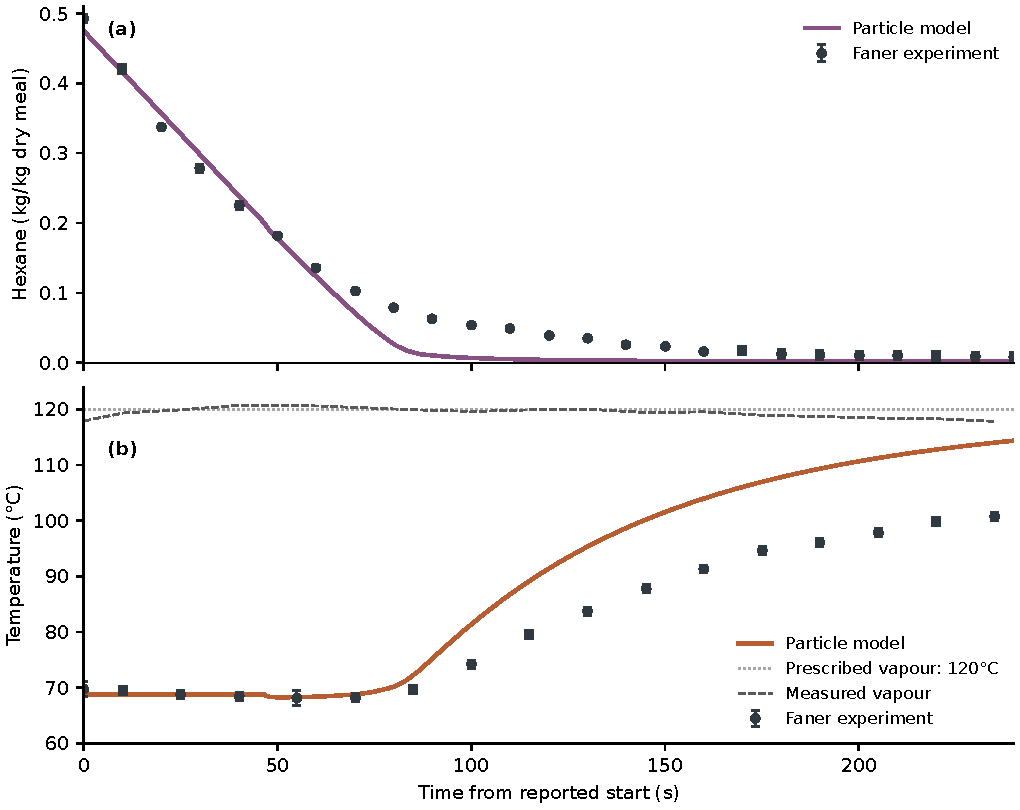
\includegraphics[width=\textwidth]{figures/fig_faner_particle_history_core2.pdf}
\caption{Faner's pure-hexane experiment: (a) hexane loading and
(b) particle temperature. Lines show calculations; markers show measurements.}
\label{fig:journalmarch}
\end{figure}

\paragraph{Solvent removal and temperature.}
External free hexane disappears at \SI{\FanerFreeEnd}{\second}; the core vanishes at
\SI{\FanerDryTime}{\second}. Loading crosses 0.20 kg/kg at
\SI{\FanerCrossTwenty}{\second} and reaches 0.10 kg/kg a further
\SI{\FanerFallingInterval}{\second} later, versus 45.9 s and 25.4 s in
the digitized source. The calculated falling interval is about
\FanerFallingShortfall\% shorter.
At 240 s, hexane is $\FanerExitHexane$ kg/kg dry, water is
$\FanerExitWater$ kg/kg dry and mean temperature is
\SI{\FanerExitTemperature}{\celsius}.
This discrepancy cannot be assigned to one mechanism: the particle sizes
are known only as summaries, the initial moisture is unknown, and the local
exposure and the thermocouple sampling are uncertain.
Table~\ref{tab:journalmarch} summarizes the comparison; loading crossings
are interpolated between successive calculated states. Its temperature
comparison retains the distinction between local holder and particle mean.

\begin{table}[htbp]\centering\small
\caption{Faner comparison on the reported experimental clock.}
\label{tab:journalmarch}
\begin{tabular}{@{}lrr@{}}\toprule
Observable & Faner experiment & Particle model\\\midrule
Time to $X_{\mathrm h}=0.20$, s & 45.9 & \FanerCrossTwenty\\
Interval $0.20\to0.10$, s & 25.4 & \FanerFallingInterval\\
Liquid-core disappearance, s & Not measured & \FanerDryTime\\
Water at 240 s, kg/kg dry & Not reported & \FanerExitWater\\
Temperature at 235.1 s, $^\circ$C & 100.8 & \FanerLastHolderClockTemperature\\
\bottomrule\end{tabular}\end{table}

Using the reported mean diameter instead of the smaller sphere inherited
from earlier calculations delays removal and warming: the external area per dry mass decreases and
the internal transport distances increase. This improves the loading
crossing while leaving a falling-rate discrepancy. At matched four-cell
resolution, the 80--100$^\circ$C temperature milestones occur about
12--17 s later than with the inherited smaller sphere. In a DT heat balance,
that timing determines how long the heat supply goes mainly to evaporation
before the meal warms, affecting residence requirements and product quality.
The source-mean two-cell march loses its core at 90.1 s; the four-cell
value is \SI{\FanerDryTime}{\second}. Their positive-core step sequences
also differ, so this comparison is a resolution sensitivity rather than
a continuum limit.

The measured vapour varies from 117.8 to \SI{120.7}{\celsius}, rather than
remaining exactly at its nominal value. A separate two-cell sensitivity
applies that trace after core depletion and gives \SI{113.0}{\celsius}
at 240 s, compared with \SI{114.3}{\celsius} under constant vapour
temperature. The small improvement supports treating heat-supply
variation as an experimental uncertainty; it does not close the full
temperature discrepancy. Before core depletion, this sensitivity still
uses the nominal bath (Sec.~\ref*{S-sup:fanerassumptions}).
Startup calculations at higher initial moisture, 0.050 and 0.100 kg/kg,
are not yet resolved (Sec.~\ref*{S-sup:journalmarch}).

\subsection{Particle destiny in the prescribed DT bath}
\label{sec:validation:dtmarch}\label{sec:validation:otherchecks}
\label{sec:validation:uptake}\label{sec:validation:tail}\label{sec:validation:bp}
\label{sec:validation:envelope}\label{sec:validation:rewetting}\label{sec:validation:derived}
\paragraph{Bath and initial state.}
The DT experiment uses an effective spherical radius $\Rp=\SI{1.5}{\milli\metre}$
and follows the particle from feed to the prescribed exit at
\SI{1766.5}{\second} (29.4 min). This radius is the coarse end of the
previous size screening. It is consistent with the upper end of the
0.5--1.5-mm equivalent-radius range containing 95.1\% of Faner's soybean
particles \citep{faner2019kinetics}, but is not a measured DT mean.
The longer heat path and smaller surface area per unit mass make this a
useful coarse-particle case when examining residence needed for solvent
removal. It does not represent a mass-weighted meal size distribution.

Initial temperature is \SI{49.0}{\celsius}, hexane and water loadings are
0.388 and 0.124 kg/kg dry meal, and oil mass fraction is 0.0137.
The feed is cooler than the 57--60$^\circ$C examples reported by
\citet{witte_nd_soybeanmeal} and \citet{kemper2013solvent}, so sensible
heating remains part of this experiment. The selected temperature is a
scenario input, rather than a measurement for the simulated charge.
The pre-desolventizing (PD) bath is at \SI{72.0}{\celsius} with hexane mole
fraction 0.664, exposure fraction 0.00408 and indirect heat supply
85 W/kg dry until \SI{490.2}{\second}. Steam contact then leads to a
toasting bath ending at \SI{105.0}{\celsius}. The prescribed gas history
is detailed in Sec.~\ref*{S-sup:dtmarch}.

The sequence represents indirect pre-desolventizing followed by live-steam
contact, as described by \citet{kemper2013solvent}. Indirect heating removes
solvent before steam contact and reduces the solvent load on the
steam-heated trays. The selected exposure fraction approximates the small
exposed area of a bed compared with the summed areas of isolated spheres.
This exposure fraction, the imposed duty and the bath ladder together
define the experiment; they do not identify a measured industrial
operating point.
Liquid-water imbibition uses the closure of
Section~\ref{sec:model:liquidcontact}, with liquid contact conductance
0.32 mol/(m$^2$ s), derived from the uptake time of solvent-extracted meal
in liquid water, and total dry-shell retained-water mobility 1000 times
the reference retained-water mobility, the water-filled-pore limit. Both inputs were set
before and independently of the DT outlet.

\paragraph{Liquid depletion, condensation and imbibition.}
At PD exit, about 0.169 kg external free hexane/kg dry remains. It disappears
approximately 2.1 s later while the external water film accumulates.
The initial two-liquid surface equilibrium is near \SI{61.3}{\celsius};
it differs from pure hexane's boiling point. The dry shell forms at
492.3 s and core extinction occurs at 503.6 s, approximately 11.3 s after
external free-hexane depletion. Retained hexane and pore gas then
continue to evolve in regime C. Both the rapid surface evaporation and the
core recession follow from the coupled balances.

At core extinction, the particle contains 0.136 kg water/kg dry and the
external water film contains a further 0.086 kg/kg dry. The film remains
until 624.5 s, about two minutes after dry-shell formation. Liquid-water
imbibition and evaporation back to the bath compete for this inventory;
condensation does not imply that all incoming water remains in the particle.
The external water film supplies mass and energy for several minutes and
persists into regime C.

Figure~\ref{fig:dtmarch} presents wet-basis hexane and moisture alongside
the volume-mean particle temperature. Dashed curves use the right axes
for the prescribed bath mole fractions and temperature. The lower
timeline identifies pre-desolventizing and main trays; dotted vertical
lines mark A--B and B--C. The insets resolve the brief core recession
and the external water film. Green markers at 30 min show published
outlet ranges: 16--22\% moisture from Witte and 100--500 ppm solvent
and 105--110$^\circ$C temperature from Kemper
\citep{kemper2013solvent,witte_nd_soybeanmeal}. They provide industrial
context rather than paired measurements of this prescribed bath.
The calculated history ends at 29.4 min.

\begin{figure}[htbp]\centering
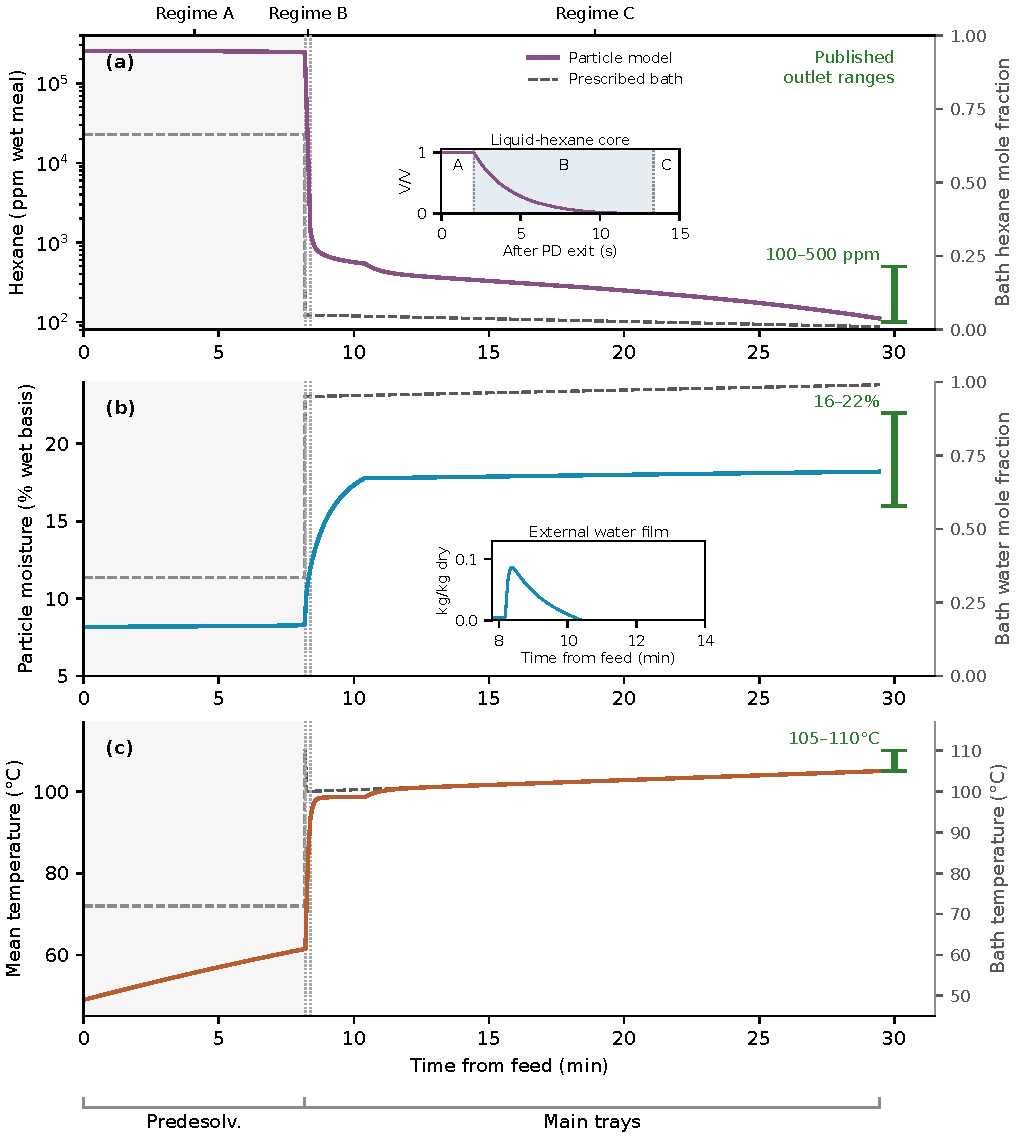
\includegraphics[width=\textwidth]{figures/fig_dt_particle_history_core2.pdf}
\caption{DT particle destiny: (a) hexane, (b) moisture and (c) temperature.
Solid lines show the particle response; dashed lines show the bath.
Green markers indicate published outlet ranges.}
\label{fig:dtmarch}
\end{figure}

\paragraph{Exit observables and numerical sensitivity.}
Particle water at exit is 0.223 kg/kg dry meal, equivalent to 18.2\%
wet-basis moisture. Hexane is 135 mg/kg dry, or 111 ppm on a wet basis, and
volume-mean particle temperature is \SI{105.0}{\celsius}.
The external water film is depleted. The particle-only basis conversion
uses $1+X_{\mathrm w}+X_{\mathrm h}$; water in the external water film is reported
separately while the film is present.
Table~\ref{tab:dtmarch} compares the result with the published outlet
ranges. Calculated ppm uses wet meal; the source solvent range does not
specify its analytical mass basis. The calculation uses two radial cells
and a 5-s maximum regime-C timestep.

\begin{table}[htbp]\centering\small
\caption{DT exit results and published outlet ranges.}
\label{tab:dtmarch}
\begin{tabular}{@{}lrl@{}}\toprule
Observable & Particle model & Published range\\\midrule
Hexane, mg/kg dry & 135 & Mass basis not specified\\
Hexane, ppm wet & 111 & 100--500\\
Particle moisture, \% wet & 18.2 & 16--22\\
Volume-mean temperature, $^\circ$C & 105.0 & 105--110\\
External water film, kg/kg dry & 0 & Not measured\\
\bottomrule\end{tabular}\end{table}

The calculated outlet lies within the published ranges. This agreement
cannot identify the imbibition coefficients or validate the prescribed bath.
In the reference case at $K_\ell=0.10$ mol/(m$^2$ s), halving the
regime-C maximum timestep from 10 to 5 s changes moisture by
0.022 percentage points, hexane by 0.52\%, temperature by 0.0016 K and
water-film depletion time by 1.8 s. The regime-B history is unchanged in
this check; full-history mesh convergence is not yet established
(Section~\ref{sec:discussion:limits}).
An independent reconstruction of every accepted advance from dry-shell
formation to exit gives maximum normalized water, hexane and energy
defects of $4.24\times10^{-11}$, $8.61\times10^{-13}$ and
$6.16\times10^{-12}$, respectively. The earlier feed audit is retained separately. The coupled
result closes the stated balances; the material transport rates
remain to be identified independently.

\section{Discussion}\label{sec:discussion}\label{sec:discussion:scope}
\label{sec:discussion:coefficients}\label{sec:discussion:refusal}\label{sec:discussion:envelope}
The two prescribed-bath experiments show how a common particle
formulation connects external-liquid evaporation, internal-core recession
and residual-component transport. Their signed component and energy
exchanges can supply a future tray calculation. Prescribing the bath
isolates this particle response, while leaving countercurrent vapour,
wall, residence and discharge balances to the equipment model. We first
interpret the Faner comparison, then its meaning for DT practice and what
is needed next.

The calculated Faner particle still dries faster than the measured
charge. Geometry is particularly consequential: image-analysis
particle counts cannot be used directly as dry-mass weights, and a volume-equivalent sphere has a
different surface area from an irregular flake of equal volume. For a
number distribution $p_n(d)$ and common density, the corresponding
mass distribution is proportional to $d^3p_n(d)$. A lognormal family
constrained by the reported mean, range and 1--3-mm fraction provides
a reproducible sensitivity construction, but does not recover the
unreported histogram. Its larger-particle mass fraction can prolong
drying even when small particles heat earlier. The direction and size
of the resulting temperature change must come from class-resolved
integration and the actual thermocouple sampling, rather than from
weights selected to obtain a desired displacement of the curves.

Faner reports preheating, so the observed lack of an initial
warming stage has an experimental basis. The exact initial temperature
and measurement trigger are not specified. A slightly subcooled start
would be a different initial-value experiment, with sensible
heating included in the balances; it cannot be represented by shifting
the calculated temperature alone. The single-particle volume mean also
does not determine the temperature of a holder probe. Simultaneous
loading, spatial temperature and size-resolved observations would help
separate startup, heat exposure and internal transport effects.

For DT practice, the three regimes divide the heat demand.
Indirect heating in PD removes external free hexane before live-steam
contact; steam condensation then supplies heat for rapid solvent removal,
and the remaining retained hexane determines the later approach to the
outlet residual. Industrial DT residence and heat supply must serve these
successive needs \citep{kemper2013solvent}. At the same time, the moist heat
treatment must reduce antinutritional activity while preserving useful
protein quality \citep{witte_nd_soybeanmeal,mustakas1981critical}.
The calculated temperature and moisture histories describe that exposure;
a meal-quality kinetic model is outside the present scope.

The moisture result also matters for energy design: water retained
at DT exit contributes to the load on the downstream dryer, which takes
meal towards its storage moisture \citep{witte_nd_soybeanmeal}.
More condensation can accelerate heat supply and solvent removal, while
more retained water can increase later drying duty. A steam-saving claim
therefore requires the full balance of steam, indirect heat and drying
energy, rather than outlet solvent or moisture alone. These prescribed-bath
experiments expose that coupling without quantifying a plant steam saving.

Two independent equilibrium checks give further context for DT practice.
At literature-motivated last-tray compositions, the dry-shell hexane equilibrium floor is
4.5--66.0 ppm without the separate oil-solution sensitivity and
8.1--112.4 ppm with it (Sec.~\ref*{S-sup:desolventizerfloor}). These
equilibrium quantities do not set the residence needed to reach them.
For retained water the diagnostic relation
\begin{equation}
\aw(\Xw)P_{\mathrm{sat}}^{\mathrm w}(T^*)=P
\label{eq:sorbedbp}
\end{equation}
gives a sorption-elevated boiling range of 100.5--\SI{107.6}{\celsius}.
It combines moisture and temperature observations from different sources;
at the moisture of the temperature study, its prediction is 2.1 K above
the observation (Sec.~\ref*{S-sup:envelopescoring}). Neither this check
nor the calculated DT exit moisture is a validation of the
coupled transient particle or the industrial tower.

In the DT history, condensate wets accessible hexane-depleted material, and a
finite pathway transfers it into the existing retained-water inventory.
Experiments by \citet{jovanovich2003wateruptake} distinguish liquid-water
imbibition from vapour sorption and show that it can include capillarity,
matrix hydration and loosely held interstitial water. Their measurements concern
protein isolates at \SI{20}{\celsius}, not extracted meal in a hot DT.
They motivate an effective liquid-connected pathway but do not supply
our coefficient, justify its 1000-fold mobility enhancement, or establish
that all absorbed liquid is molecularly bound. The present closure keeps
one capacity-bounded retained-water inventory and does not resolve those
microscopic partitions.

The imbibition closure also omits water-induced pore displacement, a
hydraulic saturation front, swelling and extra resistance to hexane escape.
In particular, the external water film is assumed permeable to hexane
without an additional transport resistance
(Section~\ref{sec:model:waterfilm}). Because the film persists for a
substantial time in the finite-contact case, this assumption has
experimental consequences. Independent transient uptake measurements on
the actual extracted meal, with external liquid quantified separately and
several particle sizes, are needed to identify the contact and internal
resistances. Closer agreement with an outlet moisture range alone would
not identify them.

\label{sec:discussion:extrapolation}\label{sec:discussion:geometry}\label{sec:discussion:limits}
Material and numerical limits set the present scope.
The analytic water isotherm
is extrapolated below its original 0.023 kg/kg anchor. Hexane retention
and binary gas cross properties also have temperature and composition
limits, and the transport coefficients are not yet identified from
simultaneous water--hexane measurements. Radius and porosity are fixed. The isobaric
pore closure omits a total-vapour Darcy/Knudsen resistance and assumes
drainage of an immobile connected liquid-hexane core. Numerically, the
two-cell DT and four-cell Faner histories provide complete discrete
experiments, but operator verification and selected timestep checks do not
yet establish whole-history continuum convergence.

\section{Conclusions}\label{sec:conclusions}\label{sec:discussion:measurements}
One conservative particle formulation completes both a 240-s
water-bearing particle experiment in pure superheated hexane and a
1766.5-s prescribed DT history. Component and energy balances
continue through external-liquid depletion, internal-front recession and
core extinction. External condensate is stored separately and exchanges
water and energy with the particle and the prescribed gas.

The declared Faner particle falls from 0.20 to 0.10 kg hexane/kg dry meal
in \SI{\FanerFallingInterval}{\second}, compared with 25.4 s measured. The DT calculation includes liquid-water imbibition
and reaches 18.2\% wet-basis moisture, 111 ppm wet-basis hexane and a
volume-mean particle temperature of \SI{105.0}{\celsius}. Its liquid
contact conductance is derived from one same-material uptake time and its
liquid-water mobility is a declared literature limit; neither is measured
on DT meal.

The model's signed water, hexane and energy fluxes can be coupled to tray
balances for DT design; in that coupled form the formulation is the
particle-level basis for a DT digital twin that can shorten process
design and support model-based control. The results connect the model's
mechanisms to observable trajectories and show which independent
geometry, uptake and temperature measurements are needed before it is
used for predictive equipment calculations.


\section*{Author contributions (CRediT)}
Tom\'a\v{s} Svoboda: Conceptualization; methodology; software; formal
analysis; validation; writing -- original draft; writing -- review and
editing. Marcela Slukov\'a: Funding acquisition; resources; supervision;
writing -- review and editing. Svatopluk Henke: Conceptualization;
methodology; writing -- original draft. Tom\'a\v{s} Moucha: Investigation;
writing -- review and editing. All authors have read and approved the
submitted manuscript.

\section*{Acknowledgments}
This research received no specific grant from any funding agency in the
public, commercial, or not-for-profit sectors.

\section*{Supplementary material}
The submitted Supplementary Material, Secs.~\ref*{S-sup:derivations}
to~\ref*{S-sup:deposit}, gives the regional and interface derivation,
property and benchmark provenance, measured-curve scoring conventions,
numerical acceptance and observed convergence results, including the
unfavorable cases. An extended technical report retains
the longer derivations, former full manuscript passages and research
history; no main-text claim relies on that report alone.

\section*{Data availability}
The governing balances, parameters, comparison conventions and numerical
acceptance criteria are stated in the text, the tables and the submitted
Supplementary Material. The particle-model source, the scripts that
produced the two particle histories and the sensitivity cases, the run
records behind every figure and printed number, and the LaTeX sources are
released at \url{https://github.com/tomas3svoboda/dt_particle_model}
(tag \texttt{v1.0.0-submission}, with a SHA-256 manifest of every file);
a preservation archive with a persistent identifier is being prepared.
Digitized readings of published figures are shared subject to the
publishers' redistribution terms, with reading half-widths and provenance.
The steady equipment-model calculation that supplies the prescribed bath
of Section~\ref{sec:validation:dtmarch} is not part of the release, but
its output is. Numerical material that does not yet exist is listed in
Section~\ref{sec:discussion:limits} and Sec.~\ref*{S-sup:missingfull};
it is not described as available.

\section*{Declaration of generative-AI assistance}
The authors used AI assistants for language editing, code review and
manuscript organization. All physical assumptions, equations, numerical
results, claim boundaries and conclusions were formulated, checked and are
owned by the authors.

\section*{Conflict of interest}
Tom\'a\v{s} Svoboda is affiliated with the University of Chemistry and
Technology Prague and with Siemens, s.r.o., of which he is an employee;
Siemens, s.r.o. had no role in the design of the study, the analysis or
the decision to publish. The other authors declare no competing interests.

\clearpage
{\footnotesize
\setlength{\parindent}{0pt}
\setlength{\columnsep}{16pt}
\newcommand{\nomblock}[1]{\par\smallskip{\small\itshape #1}\par\nopagebreak\smallskip\nopagebreak}
\newcommand{\nomitem}[2]{\par\hangindent=1.5em\hangafter=1 #1\enspace #2\par}
\section*{Nomenclature}\label{sec:nomenclature}
\begin{multicols}{2}
Symbols of the equations of this paper, with their SI units; a symbol whose
unit depends on the context gives both. Loadings are per kilogram of dry,
water- and solvent-free composite meal. Symbols used only in the
Supplementary Material are listed there.

\nomblock{Latin symbols}
\nomitem{$A_{1}$}{capacity parameter of the modified Luikov water isotherm \eqref{eq:luikov}; \si{\kilogram\per\kilogram}}
\nomitem{$A_{2}$}{shape parameter of the modified Luikov water isotherm \eqref{eq:luikov}; dimensionless}
\nomitem{$a^{*}$}{pressure-feasible n-hexane activity \eqref{eq:aceiling}; dimensionless}
\nomitem{$\ah$}{n-hexane activity; dimensionless}
\nomitem{$\aw$}{water activity; dimensionless}
\nomitem{$\bar{h}_{k}$}{partial enthalpy of component $k$ on the common caloric datum, per mole; $\bar{h}_{\mathrm{h,d}}$ that of n-hexane on the dry side; \si{\joule\per\mole}}
\nomitem{$B$}{Darcy permeability of the particle pore space \eqref{eq:darcy}; \si{\square\metre}}
\nomitem{$\Bh$}{binding potential of n-hexane, per kilogram of dry meal \eqref{eq:wetenergy}; \si{\joule\per\kilogram}}
\nomitem{$C$}{GAB energy constant in \eqref{eq:gab}; dimensionless}
\nomitem{$c$}{molar density of the pore gas, in $\Lwh = c\,\yw\yh D_{b}$; \si{\mole\per\cubic\metre}}
\nomitem{$c_{\mathrm{h,g}}$}{n-hexane mass concentration in the pore gas; \si{\kilogram\per\cubic\metre}}
\nomitem{$c_{p}$}{specific heat capacity at constant pressure; \si{\joule\per\kilogram\per\kelvin}}
\nomitem{$C_{\mathrm{h,d}}^{\Gamma}$, $C_{\mathrm{h,w}}^{\mathrm{b}}$}{n-hexane concentration at the dry-side equilibrium interface trace, and in the wet-side donor state \eqref{eq:frontvelocity}; \si{\mole\per\cubic\metre}}
\nomitem{$C_{k}$}{total local concentration of component $k$ over all of its phases; \si{\mole\per\cubic\metre}}
\nomitem{$c_{\mathrm{w}}$}{constant shift of the caloric zero of water \eqref{eq:gauge}; \si{\joule\per\mole}}
\nomitem{$\Deff$}{effective diffusivity of n-hexane in the separate Fickian comparison, Eq.~(\ref*{S-eq:ficklimit}); \si{\square\metre\per\second}}
\nomitem{$D_{b}$}{binary pore coefficient of the mobility $\Lwh$; \si{\square\metre\per\second}}
\nomitem{$d_{p}$}{mean equivalent particle diameter in the dispersion estimate; \si{\metre}}
\nomitem{$e_{\mathrm{w}}$}{specific energy of the liquid-hexane core, per kilogram of dry meal \eqref{eq:wetenergy}; \si{\joule\per\kilogram}}
\nomitem{$f_{\mathrm{exp}}$}{fraction of particle surface exposed to the external gas film in the prescribed DT bath experiment; dimensionless}
\nomitem{$h$, $a$, $h a$}{external film coefficient per unit particle area; specific external area per dry mass; and their product, the film supply per kilogram of dry meal; \si{\watt\per\square\metre\per\kelvin}; \si{\square\metre\per\kilogram}; \si{\watt\per\kilogram\per\kelvin}}
\nomitem{$h_{\mathrm{dm}}$}{specific enthalpy of the dry composite meal; \si{\joule\per\kilogram}}
\nomitem{$\Delta P$}{pore-gas overpressure across the dry shell \eqref{eq:darcy}; \si{\pascal}}
\nomitem{$h_{\mathrm{w,l}}$}{specific enthalpy of liquid water; \si{\joule\per\kilogram}}
\nomitem{$j_{\mathrm{dm}}$, $j_{L_{\mathrm{o}}}$}{fluxes of the immobile dry meal and residual oil, zero in \eqref{eq:localenergy}; \si{\kilogram\per\square\metre\per\second}}
\nomitem{$\JE$}{total radial energy flux; \si{\watt\per\square\metre}}
\nomitem{$J_{i}$}{binary exchange flux of component $i$ in the pore gas, $J_{\mathrm{w}} = -J_{\mathrm{h}}$ \eqref{eq:binaryflux}; \si{\mole\per\square\metre\per\second}}
\nomitem{$j_{k}$}{radial flux of component $k$; \si{\mole\per\square\metre\per\second}}
\nomitem{$\mathcal L_\ell$, $K_\ell$}{additional retained-water shell mobility and finite liquid-contact conductance; \si{\mole\per\metre\per\second}; \si{\mole\per\metre\squared\per\second}}
\nomitem{$K$}{GAB constant \eqref{eq:gab}; dimensionless}
\nomitem{$k$}{component index, $k \in \{\mathrm{w},\mathrm{h}\}$}
\nomitem{$k_{\mathrm C}$}{regime-C particle-mean hexane relaxation rate, $15\Deff/\Rp^2$; \si{\per\second}}
\nomitem{$k_{\mathrm{dry}}$}{thermal conductivity of the dry shell; \si{\watt\per\metre\per\kelvin}}
\nomitem{$k_m$}{packed-bed external gas-film mass-transfer coefficient in the prescribed DT bath experiment; \si{\metre\per\second}}
\nomitem{$L$}{half-thickness of a plane flake; \si{\metre}}
\nomitem{$\Lwh$}{binary pore mobility \eqref{eq:binaryflux}; $L_{\mathrm{wh}}^{-}$, $L_{\mathrm{wh}}^{+}$ its lower and upper bound; \si{\mole\per\metre\per\second}}
\nomitem{$\Lwr$}{retained-matrix water mobility \eqref{eq:retflux}; $L_{\mathrm{w,ret}}^{-}$, $L_{\mathrm{w,ret}}^{+}$ its lower and upper bound; \si{\mole\per\metre\per\second}}
\nomitem{$M_{\mathrm w}$}{molar mass of water; \si{\kilogram\per\mole}}
\nomitem{$N_{i}^{\mathrm{g}}$}{pore-gas molar flux of component $i$ \eqref{eq:retflux}; \si{\mole\per\square\metre\per\second}}
\nomitem{$\Nt$}{total (Stefan) molar flux of the pore gas; \si{\mole\per\square\metre\per\second}}
\nomitem{$N_{\mathrm{w,ret}}$}{retained-matrix water flux \eqref{eq:retflux}; \si{\mole\per\square\metre\per\second}}
\nomitem{$N_{\mathrm w}^{\mathrm{film}}$}{outward-positive water molar flux across the external gas film in the prescribed DT bath experiment, negative for condensation; distinct from $N_{\mathrm{w,ret}}$; \si{\mole\per\square\metre\per\second}}
\nomitem{$P$}{total pressure; \si{\pascal}}
\nomitem{$P_{\mathrm{sat}}^{\mathrm{h}}$, $P_{\mathrm{sat}}^{\mathrm{w}}$}{vapour pressure of n-hexane and of water; \si{\pascal}}
\nomitem{$q$}{radial conductive heat flux; \si{\watt\per\square\metre}}
\nomitem{$Q_{\Gamma}$}{swept-volume rate of the front \eqref{eq:sweptvolume}; \si{\cubic\metre\per\second}}
\nomitem{$R$, $R_{\mathrm{g}}$}{molar gas constant; \si{\joule\per\mole\per\kelvin}}
\nomitem{$r$}{radial coordinate; \si{\metre}}
\nomitem{$r_1(t)$, $r_2(t)$}{moving inner and outer radii of a spherical control volume in \eqref{eq:movingcomp}--\eqref{eq:movingenergy}; \si{\metre}}
\nomitem{$r_{\mathrm{pore}}$}{pore radius in the capillary-bundle permeability; \si{\metre}}
\nomitem{$R_{E}$, $R_{\mathrm{w}}$}{discrete energy and water residuals of the interface rows \eqref{eq:gauge}; \si{\watt}; \si{\mole\per\second}}
\nomitem{$\Rp$}{particle radius; \si{\metre}}
\nomitem{$\front$}{radius of the evaporation front; \si{\metre}}
\nomitem{$\dot{\front}$}{front velocity, negative while the front recedes; \si{\metre\per\second}}
\nomitem{$T$}{temperature; \si{\kelvin}}
\nomitem{$t$}{time; \si{\second}}
\nomitem{$\Delta t$}{time step; \si{\second}}
\nomitem{$T_{\mathrm{hex}}^{\mathrm{bp}}$}{boiling temperature of n-hexane in the flashing-zone interpolation of \citet{coletto2022modeling}; \si{\kelvin}}
\nomitem{$T_{L}$}{flashing-zone solid temperature in that interpolation; \si{\kelvin}}
\nomitem{$T_{V}$}{vapour temperature in that interpolation; \si{\kelvin}}
\nomitem{$\Tg$}{gas temperature; \si{\kelvin}}
\nomitem{$\Tint$}{interface temperature; \si{\kelvin}}
\nomitem{$T^{*}$}{boiling point of sorbed water \eqref{eq:sorbedbp}; \si{\kelvin}}
\nomitem{$u$}{total local internal energy density; \si{\joule\per\cubic\metre}}
\nomitem{$u_{\mathrm{d}}^{\Gamma}$, $u_{\mathrm{w}}^{\mathrm{b}}$}{$u$ at the dry-side equilibrium interface trace and in the wet-side donor state; \si{\joule\per\cubic\metre}}
\nomitem{$u_{\mathrm{h,l}}$}{specific internal energy of liquid n-hexane; \si{\joule\per\kilogram}}
\nomitem{$V_{\Rp}$}{particle volume; \si{\cubic\metre}}
\nomitem{$\Wret$}{retained-water loading in \eqref{eq:capcomplementarity}; \si{\kilogram\per\kilogram}}
\nomitem{$\Wcap$}{retained-water capacity, the upper end of the measured water evidence; \si{\kilogram\per\kilogram}}
\nomitem{$W_{\mathrm{eq}}$}{equilibrium retained n-hexane loading in Eq.~(\ref*{S-eq:ficklimit}); \si{\kilogram\per\kilogram}}
\nomitem{$W_{\mathrm{native}}$}{retained n-hexane on reference soybean meal \eqref{eq:gab}; \si{\kilogram\per\kilogram}}
\nomitem{$\wo$}{residual-oil mass fraction of the dry meal; dimensionless}
\nomitem{$\woref$}{residual-oil mass fraction of the reference meal, the anchor of the total-meal isotherm; dimensionless}
\nomitem{$w_{\mathrm{h}}$}{weight on the n-hexane boiling point in the flashing-zone interpolation of \citet{coletto2022modeling}; dimensionless}
\nomitem{$\Wret_{\mathrm{w}}$}{retained-water loading of the Luikov isotherm \eqref{eq:luikov}; \si{\kilogram\per\kilogram}}
\nomitem{$x$}{reduced activity $K\ah$ of the GAB isotherm \eqref{eq:gab}; dimensionless}
\nomitem{$\Xc$}{critical loading, at which mobile liquid stops reaching the outer surface; \si{\kilogram\per\kilogram}}
\nomitem{$\Xe$}{equilibrium n-hexane loading at the actual gas activity in the regime-C rate; Faner et al.'s source symbol in Eq.~\eqref{eq:faneroracle}; \si{\kilogram\per\kilogram}}
\nomitem{$\Xe^{*}$}{pressure-feasible saturated equilibrium loading at the regime-B/C boundary; \si{\kilogram\per\kilogram}}
\nomitem{$\Xf$}{external free-hexane loading; \si{\kilogram\per\kilogram}}
\nomitem{$\Xh$}{total n-hexane loading; \si{\kilogram\per\kilogram}}
\nomitem{$\Xhwa$}{apparent mobile-liquid n-hexane loading of the liquid-hexane core, set at activation and carried with the solid; distinct from the total loading $\Xh$ and from retained hexane; \si{\kilogram\per\kilogram}}
\nomitem{$X_{m}$}{GAB monolayer loading \eqref{eq:gab}; \si{\kilogram\per\kilogram}}
\nomitem{$\Xw$}{total water loading; \si{\kilogram\per\kilogram}}
\nomitem{$Y_{\mathrm w,b}$, $Y_{\mathrm w,I}$}{bulk and particle-surface gas mass fractions of water in the prescribed DT film closure; dimensionless}
\nomitem{$y_{i}$}{mole fraction of component $i$ in the pore gas; dimensionless}
\nomitem{$y_{\mathrm w,I}$, $y_{\mathrm w,b}$}{particle-surface and bulk-gas water mole fractions in the prescribed DT film closure; dimensionless}
\nomitem{$\frontz$}{wet-volume fraction $(\front/\Rp)^{3}$; $\frontz_{\mathrm{new}}$, $\frontz_{\mathrm{old}}$ at the new and old time level; dimensionless}

\nomblock{Greek symbols}
\nomitem{$\alpha$}{region label, $\mathrm{w}$ (liquid-hexane core) or $\mathrm{d}$ (dry shell)}
\nomitem{$\beta_{\mathrm{A}}$}{Ackermann blowing argument of the film law; dimensionless}
\nomitem{$\varepsilon_{\mathrm{g}}$}{gas-filled porosity of the dry shell; dimensionless}
\nomitem{$\theta_{a}$}{temperature of a material shell at activation; \si{\kelvin}}
\nomitem{$\lambda$}{multiplier of the capacity condition \eqref{eq:capcomplementarity}, a contribution to $\mu_{\mathrm{w,ret}}/(RT)$ carrying no mass, volume, enthalpy or internal energy; dimensionless}
\nomitem{$\mu_{g}$}{pore-gas viscosity \eqref{eq:darcy}; \si{\pascal\second}}
\nomitem{$\mu_{\mathrm{w}}$, $\mu_{\mathrm{h}}$, $\mu_{\mathrm{w,ret}}$}{chemical potential of water and of n-hexane in the pore gas, and of retained water; \si{\joule\per\mole}}
\nomitem{$\rho$}{gas mass density in the dispersion estimate, $(\rho c_{p})_{\mathrm{g}}$; \si{\kilogram\per\cubic\metre}}
\nomitem{$\rho_f$}{gas mass density used by the external film pair in the prescribed DT bath experiment; \si{\kilogram\per\cubic\metre}}
\nomitem{$\Cdm$}{density of the dry composite meal in the particle; \si{\kilogram\per\cubic\metre}}
\nomitem{$\tau$}{pore tortuosity in the capillary-bundle permeability; dimensionless}
\nomitem{$\phi_{i}$}{fugacity coefficient of component $i$, omitted by the ideal-gas closure; dimensionless}

\nomblock{Subscripts and superscripts}
\nomitem{$a$}{at activation}
\nomitem{$\mathrm{b}$}{donor state, the wet-core material the front sweeps (superscript); on $y_{\mathrm{w,b}}$, the bulk gas}
\nomitem{$\mathrm{c}$}{critical}
\nomitem{$\mathrm{cap}$}{capacity}
\nomitem{$\mathrm{d}$}{dry shell}
\nomitem{$\mathrm{dm}$}{dry composite meal}
\nomitem{$\mathrm{e}$, $\mathrm{eq}$}{equilibrium; $\mathrm{eq}$ on $d$: equivalent}
\nomitem{$\mathrm{eff}$}{effective}
\nomitem{$\mathrm{f}$}{external free hexane}
\nomitem{$\mathrm{g}$}{gas, pore gas}
\nomitem{$\mathrm{h}$}{n-hexane}
\nomitem{$i$, $k$}{component index}
\nomitem{$\mathrm{l}$}{liquid}
\nomitem{$m$}{monolayer}
\nomitem{$\mathrm{native}$}{reference soybean meal, at its own oil content}
\nomitem{$\mathrm{new}$, $\mathrm{old}$}{new and old time level}
\nomitem{$\mathrm{o}$}{residual oil}
\nomitem{$\mathrm{p}$}{particle}
\nomitem{$\mathrm{ref}$}{reference}
\nomitem{$\mathrm{ret}$}{retained (sorbed) phase}
\nomitem{$\mathrm{s}$}{surface; on $\mathrm{D}_{s}$, the solid}
\nomitem{$\mathrm{sat}$}{saturation}
\nomitem{$\mathrm{vap}$}{vaporization}
\nomitem{$\mathrm{w}$}{water; as a region label (on $\jump{\cdot}$, $C_{\mathrm{h,w}}$, $u_{\mathrm{w}}$), the liquid-hexane core}
\nomitem{$\Gamma$}{interface; as a superscript, the equilibrium interface trace}
\nomitem{$\alpha$}{region, $\mathrm{w}$ or $\mathrm{d}$}
\nomitem{$^{*}$}{pressure-feasible (on $a$); boiling point of sorbed water (on $T$)}
\nomitem{$^{-}$, $^{+}$}{lower and upper bound of an interval}

\nomblock{Operators and notation}
\nomitem{$\jump{\cdot}_{\mathrm{w}}^{\mathrm{d}}$}{jump across the front, dry-side value minus wet-side value}
\nomitem{$\Delta$}{a difference or a change, as in a time step or an enthalpy of vaporization}
\nomitem{$\mathrm{D}_{s}/\mathrm{D}t$}{time derivative following the solid; \si{\per\second}}
\nomitem{$\nabla$}{radial gradient; \si{\per\metre}}
\nomitem{$\partial$}{partial derivative}
\nomitem{$\dot{x}$}{time derivative of $x$}
\nomitem{$\perp$}{complementarity: both sides non-negative and their product zero}
\end{multicols}
}

\bibliographystyle{apacite}
\bibliography{refs}

\end{document}
